%% 
%% Copyright 2007-2024 Elsevier Ltd
%% 
%% This file is part of the 'Elsarticle Bundle'.
%% ---------------------------------------------
%% 
%% It may be distributed under the conditions of the LaTeX Project Public
%% License, either version 1.3 of this license or (at your option) any
%% later version.  The latest version of this license is in
%%    http://www.latex-project.org/lppl.txt
%% and version 1.3 or later is part of all distributions of LaTeX
%% version 1999/12/01 or later.
%% 
%% The list of all files belonging to the 'Elsarticle Bundle' is
%% given in the file `manifest.txt'.
%% 
%% Template article for Elsevier's document class `elsarticle'
%% with numbered style bibliographic references
%% SP 2008/03/01
%% $Id: elsarticle-template-num.tex 249 2024-04-06 10:51:24Z rishi $
%%
% Journal of Visual Communication and Image Representation
\documentclass[preprint,12pt]{elsarticle}

%% Use the option review to obtain double line spacing
%% \documentclass[authoryear,preprint,review,12pt]{elsarticle}

%% Use the options 1p,twocolumn; 3p; 3p,twocolumn; 5p; or 5p,twocolumn
%% for a journal layout:
%% \documentclass[final,1p,times]{elsarticle}
%% \documentclass[final,1p,times,twocolumn]{elsarticle}
%% \documentclass[final,3p,times]{elsarticle}
%% \documentclass[final,3p,times,twocolumn]{elsarticle}
%% \documentclass[final,5p,times]{elsarticle}
%% \documentclass[final,5p,times,twocolumn]{elsarticle}

%% For including figures, graphicx.sty has been loaded in
%% elsarticle.cls. If you prefer to use the old commands
%% please give \usepackage{epsfig}

%% The amssymb package provides various useful mathematical symbols
\usepackage{amssymb}
%% The amsmath package provides various useful equation environments.
\usepackage{amsmath}
%% The amsthm package provides extended theorem environments
\usepackage{amsthm}
\usepackage{booktabs}
\usepackage{multirow}
\usepackage{makecell}
\usepackage{tabularx}
\usepackage{arydshln}
\usepackage{subcaption}


%% The lineno packages adds line numbers. Start line numbering with
%% \begin{linenumbers}, end it with \end{linenumbers}. Or switch it on
%% for the whole article with \linenumbers.
%% \usepackage{lineno}


\usepackage{xcolor}



\newcommand{\red}[1]{\textcolor{red}{#1}}
\newcommand{\blue}[1]{\textcolor{blue}{#1}}





%% OUR PACKAGES
\usepackage{adjustbox}
\usepackage[percent]{overpic}
\usepackage{bbold}


%% ACRONYMNS
\usepackage{glossaries-extra}
\setabbreviationstyle[acronym]{long-short}



\newacronym{FR}{FR} {Full-Reference}

\newacronym{AR}{AR}{Augmented Reality}
\newacronym{IMEx}{IMEx}{immersive media experiences }
\newacronym{ISDB}{ISDB}{Integrated Services Digital Broadcasting }

\newacronym{NuSVR}{NuSVR}{Nu Support Vector Regression}
\newacronym{M-PCCD}{M-PCCD}{MPEG Point Cloud Compression Dataset}
\newacronym{WPC}{WPC}{Waterloo Point Cloud}
\newacronym{sklearn}{sklearn}{Scikit-Learn}
\newacronym{SVR}{SVR}{Epsilon-Support Vector Regression}
\newacronym{SGD}{SGD}{Stochastic Gradient Descent}
\newacronym{DISTS}{DISTS}{Deep Image Structure and Texture Similarity}
\newacronym{DL}{DL}{Deep Learning}
\newacronym{3D}{3D}{tridimensional}
\newacronym{2D}{2D}{bidimensional}
\newacronym{6DoF}{6DoF}{Six Degrees of Freedom}
\newacronym{AhG}{AhG}{Ah-Hoc Group}
\newacronym{CE}{CE}{Core Experiment}
\newacronym{CTC}{CTC}{Common Test Conditions}
\newacronym[longplural={Neural Networks}, plural=CNNs]{NN}{NN}{Neural Network}
\newacronym[longplural={Convolutional Neural Networks}, plural=CNNs]{CNN}{CNN}{Convolutional Neural Network}
\newacronym[longplural={Dynamic Point Clouds}, plural=DPCs]{DPC}{DPC}{Dynamic Point Cloud}
\newacronym[longplural={Feature Maps}, plural=FMs]{FM}{FM}{Feature Map}

\newacronym{ML}{ML}{Machine Learning}
\newacronym{GEOTEX}{geotex}{Geometrical Texture}
\newacronym{G-PCC}{G-PCC}{Geometry-based Point Cloud Compression}
\newacronym{ISO}{ISO}{International Organization for Standardization}
\newacronym{ITU}{ITU}{International Telecommunication Union}
\newacronym{HVS}{HVS}{Human Visual System}
\newacronym{JPEG}{JPEG}{Joint Photographics Experts Group}
\newacronym{IQA}{IQA}{Image Quality Assessment}
\newacronym{HEVC}{HEVC}{High Efficiency Video Coding}
\newacronym{LBP}{LBP}{Local Binary Pattern}
\newacronym{LCP}{LCP}{Local Color Pattern}
\newacronym{LLP}{LLP}{Local Luminance Pattern}
\newacronym{PCDP}{PCDP}{Perceptual Color Distance Pattern}

\newacronym{FSR}{FSR}{Frequency Selective Reconstruction}

\newacronym{PointPCA+RS}{PointPCA+RS}{PointPCA+ with Resource Streamlining}
\newacronym{CMP}{CMP}{Cubemap Projections}
\newacronym{OcM}{OcM}{Occupancy Map}

\newacronym{PCA}{PCA}{Principal Component Analysis}
\newacronym{VR}{VR}{Virtual Reality}

\newacronym{LF}{LF}{Light field}
\newacronym{LOGOCV}{LOGOCV}{Leave-One-Group-Out Cross-Validator}
\newacronym{LOOCV}{LOOCV}{Leave-One-Out Cross-Validation}
\newacronym{LOCO}{LOCO}{Leave-One-Content-Out Cross-Validation}
\newacronym{MOS}{MOS}{Mean Opinion Scores}
\newacronym{NNI}{NNI}{Neural Network Intelligence}
\newacronym{NR}{NR}{No-Reference}
\newacronym{PLCC}{PLCC}{Pearson's Linear Correlation Coefficient}
\newacronym{RMSE}{RMSE}{Root-Mean-Square Error}
\newacronym{MPEG}{MPEG}{Moving Picture Experts Group}
\newacronym{MPEG-I}{MPEG-I}{MPEG Immersive Media}
\newacronym{PSNR}{PSNR}{Peak Signal-to-Noise Error}
\newacronym{MSE}{MSE}{Mean Squared Error}
\newacronym[longplural={Point Clouds}, plural=PCs]{PC}{PC}{Point Cloud}
\newacronym{PCQA}{PCQA}{Point Cloud Quality Assessment}
\newacronym{QoE}{QoE} {Quality of Experience}
\newacronym{SOTA}{SOTA}{state-of-the-art}\newacronym{RMS}{RMS}{Root Mean Squared}
\newacronym{RR}{RR}{Reduced-Reference}
\newacronym{SROCC}{SROCC}{Spearman's Rank Correlation Coefficient}
\newacronym{SSIM}{SSIM}{Structural Similarity}
\newacronym{TMC2}{TMC2}{Test Model Category 2}
\newacronym{V-PCC}{V-PCC}{Video-based Point Cloud Compression}
\newacronym{VVQDB}{V-SENSE VVQDB}{V-SENSE Volumetric Video Quality Database}
\newacronym{VQA}{VQA}{Video Quality Assessment}
\newacronym{VS}{VS}{Voxel Size}
\newacronym{P2P}{P2P}{Point-to-Point}
\newacronym{P2Pl}{P2Pl}{Point-to-Plane}
\newacronym{Pl2Pl}{Pl2Pl}{Plane-to-Plane}
\newacronym{P2D}{P2D}{Point-to-Distribution}
\newacronym{PIQ}{PIQ}{PyTorch Image Quality}
\newacronym{PyIQA}{PyIQA}{PyTorch Toolbox for Image Quality Assessment}
\newacronym{CV}{CV}{Cross Validation}
\newacronym{KNN}{KNN}{K-nearest neighbors}
\newacronym{r-search}{r-search}{range search}

\newacronym{KD-tree}{KD-tree}{k-dimensional tree}
\newacronym{ROI}{ROI}{Region of Interest}

\newacronym{PPC}{PPC}{Processed Point Cloud}

\newacronym{PO}{PO}{Projections only}
\newacronym{QP}{QP}{Quantization Parameter}

\newacronym{RFR}{RFR}{Random Forest Regression}
\newacronym{RFE}{RFE}{Recursive Feature Elimination}

\newacronym{TT}{TT}{Transformed Target}
\newacronym{VGG}{VGG}{Very Deep Convolutional Networks for Large-Scale Image Recognition}















\journal{Journal of Visual Communication and Image Representation}

\begin{document}

\begin{frontmatter}

%% Title, authors and addresses

%% use the tnoteref command within \title for footnotes;
%% use the tnotetext command for theassociated footnote;
%% use the fnref command within \author or \affiliation for footnotes;
%% use the fntext command for theassociated footnote;
%% use the corref command within \author for corresponding author footnotes;
%% use the cortext command for theassociated footnote;
%% use the ead command for the email address,
%% and the form \ead[url] for the home page:
%% \title{Title\tnoteref{label1}}
%% \tnotetext[label1]{}
%% \author{Name\corref{cor1}\fnref{label2}}
%% \ead{email address}
%% \ead[url]{home page}
%% \fntext[label2]{}
%% \cortext[cor1]{}
%% \affiliation{organization={},
%%             addressline={},
%%             city={},
%%             postcode={},
%%             state={},
%%             country={}}
%% \fntext[label3]{}

\title{PointPCA++: Boosting PCA-based Descriptors with Quality Measurements of Cubemap Projections }

%% use optional labels to link authors explicitly to addresses:
%% \author[label1,label2]{}
%% \affiliation[label1]{organization={},
%%             addressline={},
%%             city={},
%%             postcode={},
%%             state={},
%%             country={}}
%%
%% \affiliation[label2]{organization={},
%%             addressline={},
%%             city={},
%%             postcode={},
%%             state={},
%%             country={}}

\author[1]{Arthur Henrique Silva Carvalho}
\ead{henrique-arthur.ah@aluno.unb.br}
\ead[URL]{http://lattes.cnpq.br/8280581631925622}

% Second author
\author[1]{\corref{cor1}Pedro Garcia Freitas}
% Corresponding author indication
\ead{pedro.freitas@unb.br}
\ead[URL]{https://pedrogarcia.gitlab.io/}



%% Author affiliation
\affiliation[1]{organization={Department of Computer Science, University of Brasília},
            addressline={CIC/EST Building, Campus Darcy Ribeiro, Asa Norte}, 
            city={Brasilia},
%          citysep={}, % Uncomment if no comma needed between city and postcode
            postcode={70910-900}, 
            state={DF},
            country={Brazil}}

%% Abstract
\begin{abstract}
\gls{PCQA} plays a fundamental role in 3D spatial data acquisition, compression, transmission, and rendering for human-oriented technologies. In this paper, we propose a computationally efficient enhancement of the PointPCA+ \gls{PCQA} metric, namely PointPCA++. PointPCA+ is a descriptor-based metric that employs \gls{PCA} decomposition on the geometry data and defines a set of texture descriptors to model perceptual features. The proposed PointPCA++ retains these features and also introduces an additional set of complementary features based on 3D-to-2D projections. The quality score is obtained through a learning-based method that fuses high-dimensional features to predict the visual quality of the point cloud. Extensive experimental results show that the proposed method achieves high predictive performance against subjective ground truth scores obtained from the APSIPA, ICIP2023, QoMEX2019, SJTU-PCQA, UnB, and WPC\red{2.0?} benchmark datasets. Moreover, statistical and correlation tests demonstrate that PointPCA++ significantly outperforms \gls{SOTA} \gls{PCQA} methods while demanding considerably fewer computational resources, such as memory and processing time. The code is available at https://gitlab.com/gpds-unb/projected-gats-metric.
\end{abstract}

%%Graphical abstract
\begin{graphicalabstract}
%\includegraphics{grabs}
\end{graphicalabstract}

%%Research highlights
\begin{highlights}
 \item A novel quality metric named PointPCA++ is proposed.
 \item PointPCA++ enhances PointPCA+ for improved quality assessment of point clouds.
 \item PointPCA++ offers high performance with lower memory and processing needs.
 \item PointPCA++ outperforms state-of-the-art methods on benchmark datasets.
\end{highlights}

%% Keywords
\begin{keyword}
Point cloud \sep Principal component analysis \sep Feature selection \sep Visual quality assessment
\end{keyword}

\end{frontmatter}

%% Add \usepackage{lineno} before \begin{document} and uncomment 
%% following line to enable line numbers
%% \linenumbers

%% main text
%%

%% Use \section commands to start a section
\section{Introduction}


\glspl{PC} have emerged as an essential data type for depicting 3D objects and realistic environments due to their ability to capture complex, real-world scenes with high precision. \glspl{PC} are being used as the preferred medium in a variety of applications, such as autonomous driving~\cite{LIANG2022103667}, robotics~\cite{LI2025104503}, and immersive media~\cite{WANG2024104292}. With the advancement of multimedia technology, \gls{PC} features are becoming increasingly exploited to provide enhanced applications such as \gls{VR} and \gls{AR}~\cite{WANG2024104110, LI2022103641}. To enable \gls{IMEx}, a series of challenges must be overcome—challenges that involve data acquisition, representation and compression, transmission, and the display of these media~\cite{farias2023quality}. The current industry trend favors point clouds due to their robust ecosystem, which is likely to achieve greater acceptance as computational and storage capabilities advance~\cite{perra2020an,astola2020jpeg}.

A \gls{PC} consist of a collection of points in a 3D space, often represented in Cartesian coordinates (x,y,z) with a set of attributes associated with each point. These attributes can vary, but commonly include RGB components, reflective information, physical sensor data, and normal vectors. To accurately describe a realistic 3D scene, especially for \gls{IMEx} applications, \glspl{PC} require a huge number of points.  As a consequence, coding technologies must implement lossy compression approaches to enable real applications~\cite{LUO2025104481, PAN2024104243}. Nevertheless, the main issue with using lossy compression is that it impairs the quality of the original data in order to achieve smaller file sizes, making the visual content less appealing depending on the compression level. For instance, Figure~\ref{fig_teaser} depicts a compression process that, depending on its \gls{QP}, can affect the same content in various ways. These differently compressed \glspl{PC} may influence human perception of quality in distinct ways, potentially impairing \gls{QoE} across several aspects. Consequently, the progress of these lossy compression algorithms has demanded to the development of quality assessment methods specifically designed for \gls{PC} contents.

\begin{figure*}[t!]
  \centering
  \setlength{\fboxrule}{0.5pt}
  \setlength{\fboxsep}{0pt}
  \fbox{\includegraphics[width=\textwidth]{figures/teaser.pdf}}
  \caption{ Visual effects caused by varying \acrfull{QP} of the DRACO codec~\cite{de2022quality} on the pristine point cloud.}
  \label{fig_teaser}
\end{figure*}

\gls{PCQA} has emerged as a critical research field, focusing on quantifying quality-aware features to ensure perceptual fidelity to enhance the performance of downstream tasks, such
as compression and reconstruction. \gls{PCQA} follows the same strategies used for other media signals, such as images, videos, \glspl{LF}, etc. These strategies are classified into subjective~\cite{alexiou2018pointsubjective, tious2023Physicall} and objective~\cite{Freitas2018noref, Zhou2024NoReference} categories. Subjective quality evaluation techniques assess the quality perceived by human viewers by requiring them to assign numerical opinion scores to the stimuli under assessment. The average of all viewers ratings for a given stimulus, known as the \gls{MOS}, represents the overall quality rating that an average person would attribute to that stimulus. These \gls{MOS} values are derived from psychophysical experiments. These experiments, despite being considered the most accurate way to estimate visual quality, are quite expensive and demand significant time and human resources. Therefore, subjective experiments are difficult to be used in many  scenarios. On the other hand, these psychophysical experiments are fundamental to create quality datasets for benchmark purposes. These benchmark datasets can be used to create and evaluate the objective quality assessment methods.

Objective quality assessment methods, commonly referred as `quality metrics', are techniques used to estimate the quality of visual stimuli automatically, i.e., using an algorithm that can be implemented as computer programs. Automatic quality assessment of \glspl{PC} can improve \gls{IMEx} applications by reducing the effort required to manually evaluate their quality. Metrics can be categorized based on their approach and application by determining whether they rely on a reference to assess the quality of a given point cloud. \gls{FR} metrics need to access the whole reference content at the time of assessment. \gls{FR} metrics are very useful in many contexts, but when the pristine reference \gls{PC} is not completely available, full-reference metrics can not be usable. On the other hand, \gls{RR} metrics use only partial information from the reference, while \gls{NR} metrics are able to assess the quality of a \gls{PC} without any reference information. Compared with conventional images and videos, designing \gls{PCQA} metrics is more challenging since \glspl{PC} can be sparse, disordered, and unstructured.


From a taxonomic standpoint, \gls{PCQA} metrics are classified in different ways, depending on the authors. For instance, Alexiou \& Zhou et al.~\cite{alexiou2024pointpca, zhou2023pointpca+, zhou2025pointpca+} categorize \gls{PCQA} methods as hand-crafted and learning-based features, considering that metrics are essentially composed of two components: feature extraction and regression. Smitskamp~\cite{smitskamp2022no} states that \gls{PCQA} methods can be categorized based on approaches such as projection/multi-view, (deep-)learning, histograms, topology, etc., and that \gls{FR} metrics compare point, local, or global features of a distorted \gls{PC} to the corresponding part of the original. Diniz et al.~\cite{DINIZ202231} classify the \gls{PCQA} metrics into point-to-point, point-to-plane, plane-to-plane, point-to-mesh, projection-based, and descriptor-based. Similarly, Javaheri~\cite{Javaheri-Point-cloud-quality-assessment} categorizes \gls{PCQA} metrics into point-based, feature-based, and projection-based. Yang ~\cite{yang2020predicting} and Cui et al.~\cite{Cui2024Colored} group the metrics into 3D- and 2D-based approaches.

Among the 3D-based approaches, a variety of metrics have been proposed to measure the geometric distortions of \glspl{PC}. For example, Mekuria et al.~\cite{mekuria2017performance} presented a point-to-point \gls{FR} metric to measure geometric differences by computing \gls{MSE} between equivalent points in both reference and distorted point clouds. Tian at al.~\cite{tian2017geometric} modeled the \gls{PC} surface characteristics based on tangent planes and presented a point-to-plane metric by measuring the point to plane distances in both reference and test \glspl{PC}. In a similar fashion, Alexious \& Ebrahimi~\cite{alexiou2018pointangular} introduced a plane-to-plane method based on the angular similarity between tangent planes. Javaheri et al.~\cite{javaheri2020generalized} employed generalized Hausdorff distance to model a metric to assess \glspl{PC} distorted contents. Javaheri et al~\cite{javaheri2020generalized} also introduced a geometry-only metric based on the Mahalanobis distance between points and their nearest neighbors. In addition to these metrics that consider only the geometry of the point cloud, other 3D-based approaches have been proposed to also account for additional attributes, such as color and normals. For instance, Javaheri et al.~\cite{javaheri2020improving} adapted \gls{PSNR} to measure distortions in geometry and texture in \glspl{PC}. Analogously, Alexious \& Ebrahimi~\cite{alexiou2020towards} proposed a PC-based \gls{SSIM} metric. Viola et al.~\cite{viola2020color} computed color histogram and color correlogram to assess \gls{PC} quality. Diniz et al.~\cite{Diniz2020Towards} proposed the first descriptor-based metric by modeling a 3D version of the local binary patterns descriptor. This research was further developed by exploiting multiple distance metrics to capture differences in neighborhoods~\cite{diniz2020multi}. A variant descriptor called local luminance pattern was proposed by Diniz et al.~\cite{diniz2020localluminance, diniz2021novel} with the same purposes. Also following this descriptor-based approach, Alexiou et al.~\cite{alexiou2024pointpca} proposed PointPCA, which is applied to both geometry and texture data for full-reference \gls{PCQA}. This work was extended by Zhou~\cite{zhou2023pointpca+, zhou2025pointpca+}, who employed \gls{PCA} solely on the geometry, thereby achieving improved computational efficiency.

2D-based \gls{PCQA} approaches consist of projecting the \gls{PC} onto 2D planes and subsequently handle these planes as ordinary digital images. Generally, these two-dimensional projections are produced to enable the use of established quality metrics for 2D images. In fact, 2D projection-based approaches were among the first to be proposed, as they aim to employ highly efficient image metrics in terms of perception. Moreover, since they do not require analyzing all points, they are often more computationally efficient in certain models. Torlig et al.~\cite{Torlig2018anovel} proposed a method based on 2D projections, where these projections are then employed by two-dimensional image quality metrics to predict the perceptual quality of the displayed stimuli. Alexious \& Ebrahimi~\cite{alexiou2019exploiting} extended the previous studies on projection-based objective quality assessment of \gls{PC} imagery by exploring how the number of viewpoints used influences the evaluation of visual quality. Yang et al.~\cite{yang2020predicting} projected \glspl{PC} onto a plane and then computed the texture (color) image and the corresponding depth map for quality assessment purposes. More recently, projection-based methods have been exploiting deep learning techniques that are well-established for 2D images. For example, Bourbia et al.~\cite{bourbia2022blind, Bourbia20232, Bourbia2023multi} proposed a method that projects a 3D \gls{PC} onto 2D images and then feeds these images to a deep neural network to predict the perceptual quality scores. Similar to Bourbia, Carvalho et al.~\cite{Carvalho2024perception} used deep learning to model a \gls{PC} quality metric by computing structural similarity between feature maps from a pre-trained network, but with a different approach.


%In this paper, we propose a \gls{FR} objective \gls{PCQA} metric that combines both 3D and 2D approaches. Indeed, there have already been few efforts to create hybrid models based on this 2D/3D combination. 
More recently, there have been few efforts to create hybrid models based on this 2D/3D combination. For instance, Javaheri et al.~\cite{Javaheri2022joint} proposed a joint geometry and color projection-based \gls{PC} quality metric which solves the misalignment between the reference and degraded projected images. Freitas et al.~\cite{freitas2023point} proposed calculating the visual texture similarities from the 2D projections of both the reference and degraded \glspl{PC}, and then combining them with geometric similarities to evaluate the \gls{PC} quality. Similarly, Cui et al.~\cite{Cui2024Colored} proposed a \gls{PCQA} metric using complementary 3D and 2D feature spaces to model perceptual \glspl{PC} properties. 

Unlike methods that rely solely on 2D or 3D approaches, those methods combining both have demonstrated better robustness to different distortions and improved accuracy in predicting perceptual quality scores. However, these \gls{SOTA} methods based on the combination of 2D and 3D approaches have some shortcomings. As an example, the metric proposed by Freitas et al.~\cite{freitas2023point} is based on a peculiar projection technique that represents the 3D space as 2D manifolds. That means that the projections used by Freitas, while offering the convenience of mapping all points from the 3D space onto a single 2D image, do not structure the information in a semantically or visually comprehensible for humans. On the other hand, in this paper, we employ an orthographic projection that generates six images, each corresponding to a distinct viewpoint of the \gls{PC}. In other words, our approach produces a set of 2D images that represent the objects from perspectives that are visually interpretable by humans, thereby resulting in more plausible perceptual models. Moreover, the information extracted from the 3D space is based on the descriptor-based PointPCA2 method~\cite{zhou2025pointpca+}.  We chose to rely on this approach because it offers the best trade-off between quality prediction performance and low computational cost. Additionally, it serves as a superset of features proposed in other combined methods, such as those by Cui et al.~\cite{Cui2024Colored}.

This work advances the field of \gls{PCQA} by addressing the challenge of assessing \gls{PC} quality developing a novel full-reference objective metric that combines both 3D and 2D approaches. More specifically, we improved and extended the method proposed by Zhou et al.~\cite{zhou2023pointpca+, zhou2025pointpca+}, known as PointPCA+. We chose Zhou's metric because, as far as we could find, it is the most efficient \gls{SOTA} method for predicting subjective scores. However, despite this efficiency, Zhou's metric is still quite computationally costly, which can be prohibitive in various scenarios. Therefore, one contribution of our work is a new framework to generate the same features while requiring significantly less processing time and memory consumption. Additionally, we use a hybrid approach that combines these PointPCA+ features with  a projection-based pipeline. This projection technique mitigates issues of irregularity and sparsity in the original \gls{3D} \gls{PC} domain by adapting highly efficient \gls{IQA}, originally developed for standard images, to point cloud data. Furthermore, by using projections, we avoid common limitations in feature-based metrics, such as sensitivity to noise, outliers, scale, and computational complexity. Applying \gls{PCA} on geometric data and calculating descriptors from both geometric and textural data also resolves issues typical of projection-based methods, including the loss of \gls{3D} structure, viewpoint dependence, and reductions in resolution and detail. This new method we propose is called PointPCA++.


Building upon these advances, the contributions of this paper are as follows:
\begin{itemize}
    \item A novel descriptor-based metric entitled \gls{PointPCA+RS}. This metric produces the same feature set as PointPCA+ while drastically reducing computational requirements in terms of both memory and processing time. This streamlining enables the practical use of additional complementary 2D features.
    \item A novel Cubemap projection-based metric that projects the 3D point cloud onto the six faces of a cube, generating texture regions. By applying one or more \gls{IQA} metrics to these views, a tensor of perceptual distances is obtained, effectively representing the quality of the projected data.
    \item The integration of \gls{PointPCA+RS} descriptors with cubemap-based perceptual features into a unified metric produces the proposed PointPCA++. Extensive evaluations on multiple benchmark databases demonstrate that PointPCA++ achieves superior performance compared to \gls{SOTA} methods, establishing it as a notable advancement in \gls{PCQA}.
\end{itemize}


%Such an objective metric predicts content quality automatically without human input. As a full-reference metric, it evaluates both the original and distorted content to approximate the human visual system's perception. Our approach combines projections, representing point clouds as \gls{2D} images, with the PointPCA+\cite{zhou2023pointpca+} method. This projection technique mitigates issues of irregularity and sparsity in the original \gls{3D} \gls{PC} domain by adapting highly efficient \gls{IQA}, originally developed for standard images, to point cloud data. Furthermore, by using projections, we avoid common limitations in feature-based metrics, such as sensitivity to noise, outliers, scale, and computational complexity. Applying \gls{PCA} on geometric data and calculating descriptors from both geometric and textural data also resolves issues typical of projection-based methods, including the loss of \gls{3D} structure, viewpoint dependence, and reductions in resolution and detail.

The rest of this paper is organized as follows. In Section~\ref{sec_review}, we discuss the existing work related to PCA-based \gls{PCQA} methods, their advantages and limitations. In Section~\ref{sec_proposed}, we present a detailed description of the proposed PointPCA++ and its main components, namely PointPCA+RS and \gls{CMP}. The experimental setups and the results acquired on public \gls{PC} quality databases are described in Sections~\ref{sec_setup} and \ref{sec_results}, respectively. Finally, Section~\ref{sec_conclusions} concludes the paper.


\begin{figure}[t!]
    \centering
    \begin{subfigure}[b]{\textwidth}
        \centering
        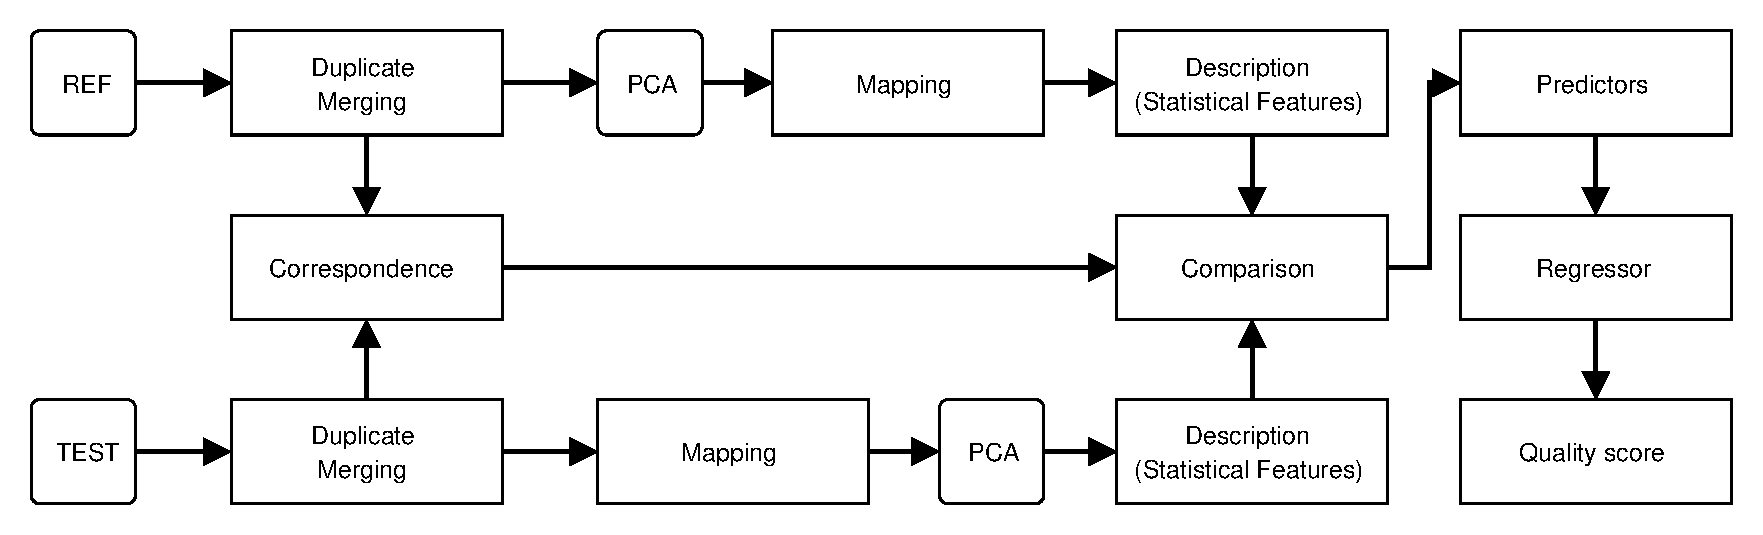
\includegraphics[width=\textwidth]{diagrams/pointpca1.pdf}
        \caption{PointPCA~\cite{alexiou2024pointpca}}
        \label{fig_pointpca_diagram}
    \end{subfigure}
    \\[1em]
    \begin{subfigure}[b]{\textwidth}
        \centering
        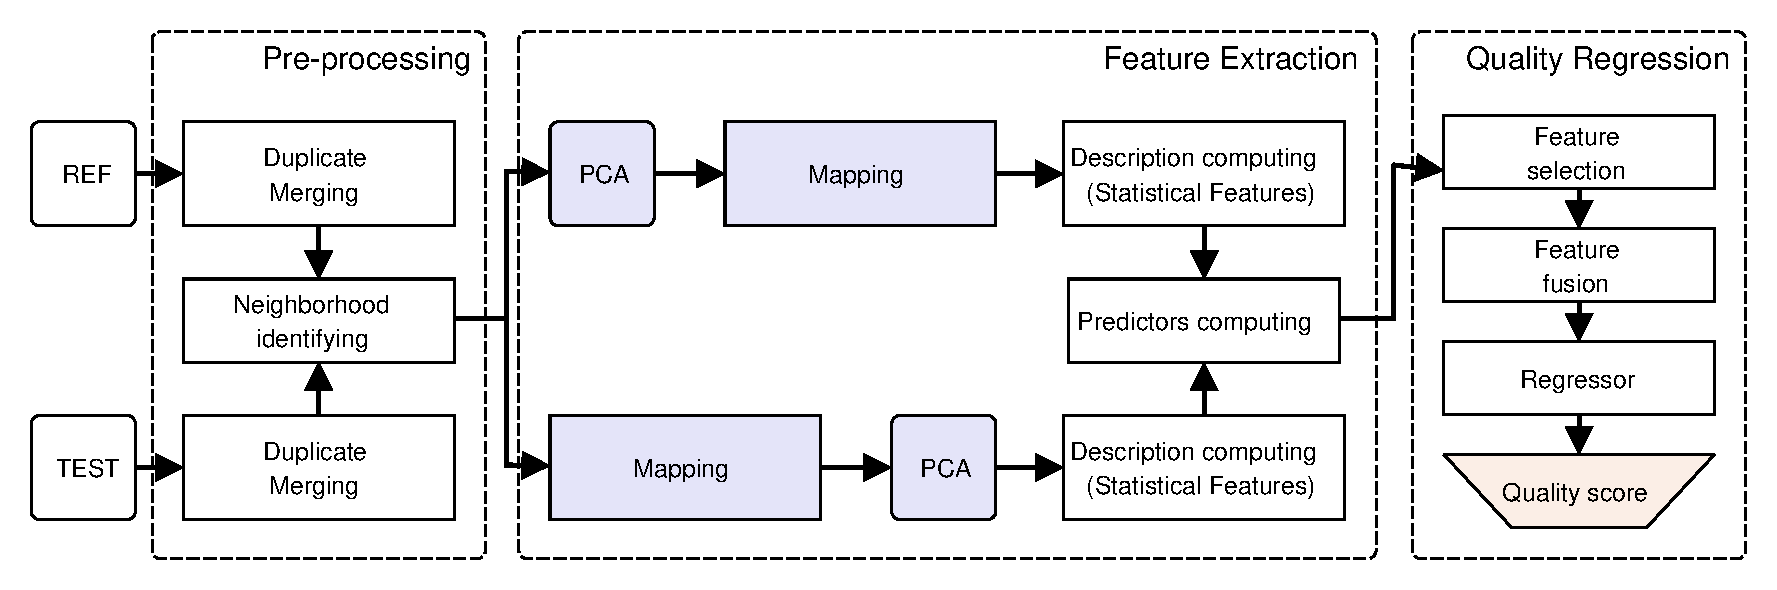
\includegraphics[width=\textwidth]{diagrams/pointpca2.pdf}
        \caption{PointPCA+~\cite{zhou2023pointpca+, zhou2025pointpca+}}
        \label{fig_pointpca2_diagram}
    \end{subfigure}
    \\[1em]
    \begin{subfigure}[b]{\textwidth}
        \centering
        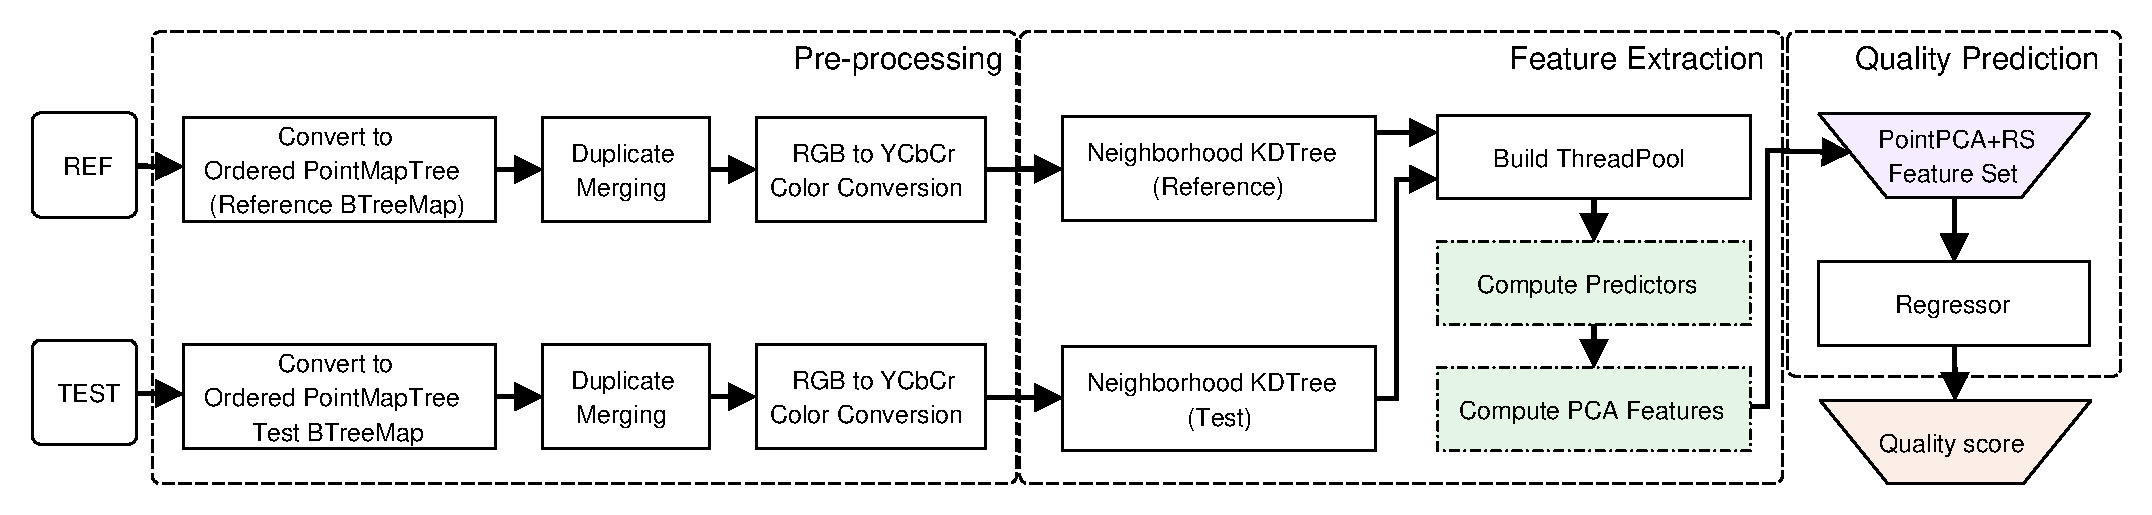
\includegraphics[width=\textwidth]{diagrams/pointpca2_rs.pdf}
        \caption{PointPCA+RS (proposed)}
        \label{fig_pointpca2_rs_diagram}
    \end{subfigure}
    \caption{Architectures of PCA-based point cloud quality assessment metrics. These metrics have some steps in common, such as duplicates merging, computation of descriptors, and statistical features. The difference between PointPCA and PointPCA+ is that PointPCA+ performs PCA only on the geometry data of the reference PC, and transforms both the reference and distorted PCs onto the new basis, avoiding costly processing operations on texture data. \gls{PointPCA+RS} is a technique proposed in this paper to generate an approximated feature set of PointPCA+ while using much less computational complexity and consuming significantly fewer computational resources.}
    \label{fig_pointpca_family}
\end{figure}




\section{A Brief Review of PCA-based Quality Descriptors} \label{sec_review}


Let a color \gls{PC} as a set of points in three-dimensional space, where each point is associated not only with spatial coordinates $(x,y,z)$ but also with color information, typically represented in a color space such as RGB. Formally, a \gls{PC} of $N$ points can be described as a set $\mathcal{P}$=$\{ (p_i \in \mathbb{R}^3, c_i \in \mathbb{R}^3) ~|~ i=1,2,\cdots,N \}$, where each point $p_i$=$(x_i,y_i,z_i)$ is associated with a color attribute $c_i=(r_i,g_i,b_i)$. Using this definition, we denote $\mathcal{A}$ as the reference \gls{PC} (depicted as `REF' in Figure~\ref{fig_pointpca_family}) from which we can find its $K$ nearest points corresponding to the distorted \gls{PC} $\mathcal{B}$ (depicted as `TEST' in Figure~\ref{fig_pointpca_family}). 

Figure~\ref{fig_pointpca_family} illustrates the three frameworks of the PCA-based family of \gls{PCQA} metrics. PointPCA~\cite{alexiou2024pointpca} was originally proposed as a seven-stage algorithm, as presented in Figure~\ref{fig_pointpca_family}-(a), with steps including duplicates merging, correspondence, descriptors, statistical features, comparison, predictors, and quality score. To predict the quality of a \gls{PC}, this metric needs a reference to compare it against. Before the comparison, any points with identical coordinates within each \glspl{PC} are merged. After merging, for each point in both \glspl{PC}, 23 geometric and textural descriptors are calculated. To capture their local characteristics, statistical functions are then applied to these descriptors, which in turn yield a set of statistical features. For each corresponding point, 46 statistical features are extracted from the reference and the evaluated \glspl{PC} and then compared. The resulting error (i.e., a difference measure) samples are aggregated to generate a quality predictor for each feature. A regression algorithm then fuses these 46 predictors to produce the final quality score.

The PointPCA process begins with the duplicate merging step, where points with identical coordinates within a single point cloud are identified and merged, retaining only one point per coordinate set. The color of the merged point is the average of the colors of the original points. This step is crucial for eliminating bias in descriptors and feature computation caused by duplicate values and for preventing redundant correspondences between \glspl{PC}.

Establishing a correspondence between two sets of points is an ill-conditioned problem. For this reason, in the correspondence step, PointPCA uses a nearest neighbor algorithm to identify correspondences between reference $\mathcal{A}$ and test $\mathcal{B}$ to favor lower complexity. Formally, the correspondence function is defined as $\mathrm{c}^{ \mathcal{B}, \mathcal{A} }:  \mathcal{B} \rightarrow  \mathcal{A}$ for $\mathrm{c}^{\mathcal{B}, \mathcal{A}} (b_i)=a_i$. Specifically, for every point $b_i \in \mathcal{B}$, a matching point $a_i \in \mathcal{A}$ is identified as the nearest neighbor in terms of Euclidean distance and is subsequently registered as its correspondence. The correspondence is not symmetric, i.e., the set of matching points obtained by finding nearest neighbors in $\mathcal{A}$ from $\mathcal{B}$ will be different from the set obtained when the roles are reversed. To ensure the result is independent of the reference choice, PointPCA uses a symmetric error approach. This approach involves setting both the pristine and impaired \glspl{PC} as references and then applying a max operation to derive the final prediction.

PointPCA defines a set of 8 textural and 15 geometric local descriptors (per point). These descriptors are extracted after applying \gls{PCA} on spatial neighborhoods of textural value and geometric coordinates. Particularly, Given a query point $p_i \not\in \mathcal{P}_i$, a surrounding support region is identified from the same \gls{PC}. This region forms a set $\mathcal{P}_i$, which consists of points $p_n \in P_i$. The covariance matrix of this set is computed as follows:
\begin{equation} \label{eq_covariance}
\mathbf{\Sigma}_i = \frac{1}{|P_i|} \sum_{n=1}^{|P_i|} ({p}_n - \bar{{p}}_i)({p}_n - \bar{{p}}_i)^\top,
\end{equation}
where $|P_i|$ is the size of the set and $\bar{{p}}_i$ represents its centroid, i.e.,
\begin{equation} \label{eq_centroid}
\bar{{p}}_i = \frac{1}{|P_i|} \sum_{n=1}^{|P_i|} {p}_n.
\end{equation}
Eigen-decomposition is performed on the covariance matrix $\mathbf{\Sigma}_i$, which is both symmetric and positive definite. As a result, its eigenvalues are non-negative and its eigenvectors form an orthogonal system. The eigenvectors represent the directions of greatest data dispersion, while the eigenvalues indicate the variance of the transformed data along these principal axes.

To compute the geometric descriptors, the coordinates of the points in $P_i$ are used. Therefore, in Equations~\ref{eq_covariance} and \ref{eq_centroid}, $p_i$ is set to $(x_i, y_i, z_i)^\top$. Assuming that $\textbf{e}_1^g$, $\textbf{e}_2^g$, and $\textbf{e}_3^g$ denote the eigenvectors and $\lambda_1^g$, 
$\lambda_2^g$, and $\lambda_3^g$ the corresponding eigenvalues ($\lambda_1^g \geq \lambda_2^g \geq \lambda_3^g$) obtained from the eigen-decomposition of $\mathbf{\Sigma}_i$. Additionally, we define the unit vectors $\mathbf{u}_x = [1, 0, 0]^\top$, $\mathbf{u}_y = [0, 1, 0]^\top$, and $\mathbf{u}_z = [0, 0, 1]^\top$ to represent the $x$, $y$, and $z$ axes. The geometric descriptors, $d^g \in \mathbb{R}^{1 \times 15}$, are constructed using these eigenvalues, eigenvectors, and unit vectors, as defined in Table~\ref{tab_pointpca_descriptors}. In this table, each descriptor represents an interpretable shape property, where $\{d_1^g, d_2^g, \cdots, d_4^g \}$ represent the individual and aggregated sum of eigenvalues that indicate the extent to which points are dispersed along the axes. The descriptors $\{d_5^g, d_6^g, d_7^g \}$  capture the dimensionality of the local surface by indicating the placements of points within a neighborhood. The descriptor $d_8^g$ highlights data variation between the first to the third principal directions. The descriptors $\{d_9^g, d_{10}^g, ~\text{and}~ d_{11}^g \}$ give a sense of the spread, uncertainty, and variation of the subjacent surface, taking into account all the main axes. The descriptor $d_{12}^g$ measures the projected distance of a query point from the centroid of its neighborhood, along the estimated normal vector $\mathbf{e}_3^g$. The remaining $d_{13}^g, d_{14}^g, ~\text{and}~ d_{15}^g$ measures the projected error of $\mathbf{e}_3^g$ onto unit vectors aligned with the Cartesian axes of the \glspl{PC} coordinate system.


\begin{table}[ht!]
\centering
\caption{Definition of PointPCA descriptors.}
\label{tab_pointpca_descriptors}
\adjustbox{max width=\columnwidth}
{
\begin{tabular}{cll}
\toprule
~ & \textbf{Descriptor} & \textbf{Definition} \\
\hline
\multirow{15}{*}{\rotatebox{90}{Geometric}} & First eigenvalue & $d_1^g = \lambda_1^g$ \\
& Second eigenvalue & $d_2^g = \lambda_2^g$ \\
& Third eigenvalue & $d_3^g = \lambda_3^g$ \\
& Sum of eigenvalues & $d_4^g = \sum_{i=1}^3 \lambda_i^g$ \\
& Linearity & $d_5^g = (\lambda_1^g - \lambda_2^g)/\lambda_1^g$ \\
& Planarity & $d_6^g = (\lambda_2^g - \lambda_3^g)/\lambda_1^g$ \\
& Sphericity & $d_7^g = \lambda_3^g/\lambda_1^g$ \\
& Anisotropy & $d_8^g = (\lambda_1^g - \lambda_3^g)/\lambda_1^g$ \\
& Omnivariance & $d_9^g = \sqrt[3]{\lambda_1^g \cdot \lambda_2^g \cdot \lambda_3^g}$ \\
& Eigenentropy & $d_{10}^g = -\sum_{i=1}^3 \lambda_i^g \cdot \ln(\lambda_i^g)$ \\
& Surface variation & $d_{11}^g = \lambda_3^g / \sum_{i=1}^3 \lambda_i^g$ \\
& Roughness & $d_{12}^g = |(p - \bar{p}) \cdot \mathbf{e}_1^g|$ \\
& Parallellity$_x$ & $d_{13}^g = 1 - |\mathbf{u}_x \cdot \mathbf{e}_1^g|$ \\
& Parallellity$_y$ & $d_{14}^g = 1 - |\mathbf{u}_y \cdot \mathbf{e}_1^g|$ \\
& Parallellity$_z$ & $d_{15}^g = 1 - |\mathbf{u}_z \cdot \mathbf{e}_1^g|$ \\
\cmidrule{2-3}
\multirow{8}{*}{\rotatebox{90}{Textural}} & Red channel & $d_1^t = R$ \\
& Green channel & $d_2^t = G$ \\
& Blue channel & $d_3^t = B$ \\
& First eigenvalue & $d_4^t = \lambda_1^t$ \\
& Second eigenvalue & $d_5^t = \lambda_2^t$ \\
& Third eigenvalue & $d_6^t = \lambda_3^t$ \\
& Sum of eigenvalues & $d_7^t = \sum_{i=1}^3 \lambda_i^t$ \\
& Eigenentropy & $d_8^t = -\sum_{i=1}^3 \lambda_i^t \cdot \ln(\lambda_i^t)$ \\
\bottomrule
\end{tabular}
}
\end{table}


Freitas et al.~\cite{freitas2023point} showed that texture measures can be more relevant for some regression models than geometry. Based on this, PointPCA uses RGB color values to serve as the first three texture descriptors, namely $d_{1}^t, d_{2}^t, ~\text{and}~ d_{3}^t$. To compute the PCA-based textural descriptors, the RGB color values of the points in $\mathcal{P}_i$ are used. Therefore, $p_i$ is set to $(R_i, G_i, B_i)^\top$  in Equations~\ref{eq_covariance} and \ref{eq_centroid}, which yields the eigenvalues  $\lambda_1^t$, 
$\lambda_2^t$, and $\lambda_3^t$, where $\lambda_1^t \geq \lambda_2^t \geq \lambda_3^t$. These eigenvalues are used as descriptors themselves, i.e., $d_4^t=\lambda_1^t$, $d_5^t=\lambda_2^t$, and $d_5^t=\lambda_3^t$. Moreover, the aggregated sum and the eigenentropy of these eigenvalues are also used as the descriptors $d_{7}^t$ and $d_{8}^t$, respectively. These descriptors are computed to measure the spread and variability of the color distribution within a local neighborhood, specifically along its principal axes. Table~\ref{tab_pointpca_descriptors} lists the formal definitions of these textural descriptors.
 

The descriptors stated above are used to compute a set of 46 features per point. Specifically, the mean is calculated to offer a smoother estimate of a surface properties, whether geometric or textural, by considering a wider region. The standard deviation is also determined to quantify how much that surface property varies within the surrounding area. In particular, considering a query point $p_i$, PointPCA identify a support region as a set $\mathbf{\widehat{P_i}}$ composed of neighboring points $p_{\hat{n}} \in \mathbf{\widehat{P_i}}$. The mean statistical feature of point $p_i$ is given by
\begin{equation} \label{eq_mean_feature}
    \mu_i(d_u^\omega) = \frac{1}{|\hat{P}_i|} \sum_{\hat{n}=1}^{|\hat{P}_i|} d_u^\omega(\mathbf{p}_{\hat{n}}),
\end{equation}
where $d_u^\omega(\mathbf{p}_{\hat{n}})$ represents a descriptor of Table~\ref{tab_pointpca_descriptors} associated with a point $\mathbf{p}_{\hat{n}}$. Correspondingly, the standard deviation feature is then obtained via
\begin{equation} \label{eq_std_feature}
\sigma_i(d_u^\omega) = \sqrt{\frac{1}{|\hat{P}_i|} \sum_{\hat{n}=1}^{|\hat{P}_i|} (d_u^\omega(\mathbf{p}_{\hat{n}}) - \mu_i(d_u^\omega))^2}.
\end{equation}
Since $\mathbf{\mu}_i = \{ \mu_i(d_1^g), \mu_i(d_2^g), \cdots, \mu_i(d_{15}^g), \mu_i(d_1^t), \mu_i(d_2^t), \cdots, \mu_i(d_8^t) \}$ and $\mathbf{\sigma}_i = \{ \sigma_i(d_1^g), \sigma_i(d_2^g), \cdots, \sigma_i(d_{15}^g), \sigma_i(d_1^t), \sigma_i(d_2^t), \cdots, \sigma_i(d_8^t) \}$ then $ \mathbf{\mu}_i \in \mathbb{R}^{1 \times 23}$ and $ \mathbf{\sigma_i} \in \mathbb{R}^{1 \times 23}$. Therefore, the complete statistical feature vector is defined as $\mathbf{\phi}_i = \left[ \mathbf{\mu}_i; \mathbf{\sigma}_i \right] \in \mathbb{R}^{1 \times 46}$.


To compute the aforementioned descriptors and statistical features, a support region is needed in PointPCA. This region is used for both geometric and textural descriptors and is determined by the spatial proximity of points. Two common methods for defining \gls{PC} neighborhoods are the \gls{KNN} and \gls{r-search} algorithms~\cite{behley2015efficient}. \gls{KNN} creates neighborhoods of a fixed size but with a variable extent, while the \gls{r-search} defines spherical volumes of a fixed radius that can contain a different number of points. 
PointPCA opted for the \gls{r-search} to estimate the descriptors because it ensures that the same surface areas are represented in both the reference and distorted stimuli. The \gls{r-search} variant provides this consistency, unlike the \gls{KNN} algorithm, which is sensitive to variations in point density. 
For instance, if a \gls{PC} is subsampled, the \gls{r-search} method identifies regions of the same size in both the original and the compromised point clouds. In contrast, the \gls{KNN} method would consider larger regions in the impaired \gls{PC}, causing the descriptor values to represent properties of surfaces with different dimensions. On the other hand, PointPCA adopts \gls{KNN} to compute the statistical features, as its operating principle is effective for revealing topological deformations. By including neighboring samples until a count of $k$ is reached, \gls{KNN} considers larger areas in a sparser, impaired stimulus and incorporates erroneous points if they have been repositioned. This results in more significant differences when compared to measurements from the pristine content. Essentially, using \gls{KNN} allows for the penalization of both point sparsity and displacement.

After independently computing the descriptors and features from the reference and assessed \glspl{PC}, as illustrated in Figure~\ref{fig_pointpca_diagram}, PointPCA uses the following correspondence function:
\begin{equation} \label{eq_comparison_funcion_pcqa}
    r_{i,j}^{\mathcal{B}, \mathcal{A}} = \frac{\left| \phi_{i,j}^{\mathcal{A}} - \phi_{i,j}^{\mathcal{B}}\right|}{\text{max}\left( \left| \phi_{i,j}^{\mathcal{A}} \right|, \left| \phi_{i,j}^{\mathcal{B}} \right| \right) + \varepsilon},
\end{equation}
where $\phi_{i,j}^{\mathcal{A}}$ and $\phi_{i,j}^{\mathcal{B}}$ denote the $j^{th}$ statistical feature of points $a_i \in \mathcal{A}$ and $b_i \in \mathcal{B}$, respectively. The value $r_{i,j}^{\mathcal{B}, \mathcal{A}}$  represents the error sample derived from $b_i$ for $1 \leq i \leq \left| \mathcal{B} \right|$ and $1 \leq j \leq 46$. $\varepsilon$ is a small constant introduced to prevent division by zero.
After repeating this computation for all points of $\mathcal{B}$, the corresponding error samples $r_{i,j}^{\mathcal{B}, \mathcal{A}}$ are elements of a matrix $R^{\mathcal{B}, \mathcal{A}}$ in the form
\begin{equation} \label{descriptor_feat}
\mathbf{R}^{\mathcal{B}, \mathcal{A}} = \begin{bmatrix}
r^{\mathcal{B}, \mathcal{A}}_{1,1} & r^{\mathcal{B}, \mathcal{A}}_{1,2} & \cdots & r^{\mathcal{B}, \mathcal{A}}_{1,46} \\
r^{\mathcal{B}, \mathcal{A}}_{2,1} & r^{\mathcal{B}, \mathcal{A}}_{2,2} & \cdots & r^{\mathcal{B}, \mathcal{A}}_{2,46} \\
\cdots & \vdots & \ddots & \cdots \\
r^{\mathcal{B}, \mathcal{A}}_{\left| \mathcal{B} \right|,1} & r^{\mathcal{B}, \mathcal{A}}_{\left| \mathcal{B} \right|,2} & \cdots & r^{\mathcal{B}, \mathcal{A}}_{\left| \mathcal{B} \right|,46} \\
\end{bmatrix}.
\end{equation}
This matrix is produced as result of the `Comparison' box depicted in Figure~\ref{fig_pointpca_diagram}. By applying a per-column pooling function, the matrix is $\left(\mathbf{R}^{\mathcal{B}, \mathcal{A}}\right)_{\left| \mathcal{B} \right|\times 46}$ is reduced to an array $\left(\mathbf{s}^{\mathcal{B}, \mathcal{A}}\right)_{1 \times 46}$ that can be used as feature vector representing the whole pair of references and test \glspl{PC}. Many summary statistics can be used pooling function to produce $\mathbf{s}^{\mathcal{B}, \mathcal{A}}$ (e.g., mean, median, sum, maximum, minimum, etc). In \cite{alexiou2024pointpca}, Alexiou et al. use an ordinary arithmetic mean for PointPCA, i.e.,
\begin{equation} \label{eq_pooling_poinpca}
    s_j^{\mathcal{B},\mathcal{A}} = \frac{1}{|\mathcal{B}|} \sum_{i=1}^{|\mathcal{B}|} r_{i,j}^{\mathcal{B},\mathcal{A}},
\end{equation}
where $s_j^{\mathcal{B},\mathcal{A}} \in \mathbf{s}^{\mathcal{B}, \mathcal{A}}$. The same calculations are repeated with \gls{PC} $\mathcal{B}$ as the reference, which produces the corresponding measurements $s_j^{\mathcal{A}, \mathcal{B}} \in \mathbf{s}^{\mathcal{A}, \mathcal{B}}$. Finally, the actual feature vector is composed by the `Predictors' box depicted in Figure~\ref{fig_pointpca_diagram}. For each statistical feature $j$, the corresponding predictor is given by $s_j=\text{max}(s_j^{\mathcal{B},\mathcal{A}}, s_j^{\mathcal{A},\mathcal{B}})$. 
Each predictor $s_j \in \left(\mathbf{s}\right)_{1 \times 46}$ provides a global quality description based on the feature $j$. The final feature vector $\mathbf{s}$ is then used as input into a regression algorithm to map these 46 predictors into a single final quality score. 


The PointPCA+ framework is outlined in Figure~\ref{fig_pointpca2_diagram}. It was proposed by the same authors of PointPCA to overcome some of its limitations, such as the high computational complexity resulting from calculating \gls{PCA} on both geometric and textural data and the need for two separate search algorithms (\gls{KNN} and \gls{r-search}). To address these shortcomings, PointPCA+ uses a richer set of simpler descriptors than its predecessor. It performs \gls{PCA} on only the geometric data of the reference \gls{PC}. By transforming both the reference and test \glspl{PC} onto a new basis, the framework substantially reduces the algorithm's complexity. Moreover, PointPCA+ employs only the \gls{KNN} algorithm to determine the neighborhood of $p_i$, further reducing the overall computational cost of the resulting metric.

Despite the similarities with PointPCA, Zhou et al.~\cite{zhou2025pointpca+} split PointPCA+ into three main modules: pre-processing, feature extraction, and quality regression. In the pre-processing stage, the duplicate merging step operates exactly as described for PointPCA: points with identical coordinates that belong to the same \gls{PC} are consolidated into a single sample. The color of this merged point is determined by averaging the colors of the duplicated points. In PointPCA+, a \gls{KNN} algorithm based on \gls{KD-tree} is used to identify neighborhood pairs between two \glspl{PC}. For each point within $\mathcal{A}$, its $N$ nearest reference points and its $N$ nearest distorted points from $\mathcal{B}$ are located using the Euclidean distance. 

The feature extraction of PointPCA+ mirrors that of PointPCA, including the computation of geometry and texture descriptors based on the identified neighborhoods to get the local quality degradations of the assessed \gls{PC}. Statistics derived from these descriptors are then used as predictors of visual quality and features are obtained by pooling these predictors. However, in contrast to PointPCA, PointPCA+ uses only the pristine \gls{PC} as a reference to find matches in the distorted \gls{PC}, saving a significant amount of computational resources. 

This means that the model presented in Equation~\ref{eq_covariance} is slightly modified to consider only the geometry of $\mathcal{A}$, rather than being computed independently for both $\mathcal{A}$ and $\mathcal{B}$, i.e.:
\begin{equation} \label{eq_covariance_pointpca2}
    \Sigma_i\mathcal{A} = \frac{1}{K} \sum_{n=1}^{K} \left( p_{n}^{g,\mathcal{A}} - \bar{p}_{i}^{g,\mathcal{A}} \right) \cdot \left( p_{n}^{g,\mathcal{A}} - \bar{p}_{i}^{g,\mathcal{A}} \right)^\top,
\end{equation}
where  $p_{i}^{g,\mathcal{A}}$ the geometry of the query point $p_i \in \mathcal{A}$ and $\bar{p}_{i}^{g,\mathcal{A}}$ is the centroid computed like in Equation~\ref{eq_centroid}.  Next, eigen-decomposition is performed on $\Sigma_i^\mathcal{A}$ to derive the eigenvectors, which constitute an orthonormal basis $V^\mathcal{A}$ made up of eigenvectors $v_m^{\mathcal{A}}$ with corresponding eigenvalues $\lambda_m^{\mathcal{A}}$, where $\lambda_1^{\mathcal{A}} > \lambda_2^{\mathcal{A}} > \lambda_3^{\mathcal{A}}$. Subsequently, the reference and distorted neighborhoods are projected onto the new orthonormal basis, expressed as $\omega_n^{\mathcal{F}} = \left( p_{n}^{g,\mathcal{F}} - \bar{p}_{i}^{g,\mathcal{A}} \right) \cdot V^\mathcal{A}$, where $p_n^{g, \mathcal{F}}$=$(x_n, y_n, z_n)^\top$ and $\mathcal{F} \in \{ \mathcal{A}, \mathcal{B} \}$. \gls{PCA} is applied to the covariance matrix of $\omega_n^{\mathcal{B}}$ to derive the eigenvectors $v_m^{\mathcal{B}}$ and eigenvalues $\lambda_m^{\mathcal{B}}$. The mapped coordinates $\omega_n^{\mathcal{F}}$, eigenvectors $v_m^{\mathcal{F}}$, and unit vector $u_m^T$ are then used to form the descriptors listed in Table~\ref{tab_pointpca2_descriptors}. 


The primary advantage of projecting both the $\mathcal{A}$ and $\mathcal{B}$ onto a shared orthonormal basis is that it unifies the representation of geometric degradation within a common space. This unification enables a more precise measurement of geometry similarity within the framework. Because of this basis change, the modeling of subsequent steps of PointPCA+ is substantially different from PointPCA, especially in the formulation of descriptors, as can be noted from the formulas listed in Table~\ref{tab_pointpca_descriptors} compared to those in Table~\ref{tab_pointpca2_descriptors}.

Each descriptor in Table~\ref{tab_pointpca2_descriptors} provides an interpretable description of the shape within the neighborhood. Specifically, $e$ represents the error vector between the mapped coordinates of the reference query point and its nearest neighbor. From this, $\epsilon_m$ is defined as the projected distance of the error vector along the m$^{th}$ principal axis. $\epsilon$ quantify the Euclidean distances of the mapped reference query point and its nearest neighbor from the centroid, as well as their projected distances from the principal axes. The remaining geometry descriptors characterize the local statistics ($\mu^\mathcal{B}$, $\lambda_m^\mathcal{F}$, $\Sigma^\mathcal{F}$) and other topological properties relying on spatial/angular dispersion and uncertainty on the projected surfaces.

Another modification in PointPCA+ compared to PointPCA relies in the texture descriptors. While PointPCA uses the R, G, and B values as texture descriptors, PointPCA+ converts the color space from RGB to YCbCr, denoting the texture information of $p_i$ as $p_n^{t,\mathcal{F}} = \left( Y_n, Cb_n, Cr_n \right)^\top$. This conversion is based on the principle that the \gls{HVS} is more sensitive to changes in brightness than to changes in color. 

While PointPCA defines 8 texture descriptors, the 6 texture descriptors of PointPCA+ express the distribution of luminance and chromatic components of YCbCr channels ($\tilde{\mu}^\mathcal{F}$, $\tilde{g}^\mathcal{F}$, and $\tilde{\Sigma}^\mathcal{F}$) and the variability of color information ($\tilde{\Sigma}$, $\tilde{\mathcal{O}}^\mathcal{F}$, and $\tilde{\mathcal{H}}^\mathcal{F}$). In the same way as for the geometry descriptors, each texture descriptor is computed per point $p_i$.



\begin{table}[t]
\centering
\caption{Definition of PointPCA+ descriptors.}
\label{tab_pointpca2_descriptors}
\adjustbox{max width=\columnwidth}
{
\begin{tabular}{cllc}
\toprule
~ & \textbf{Descriptor} & \textbf{Definition} & \textbf{Distance} \\
\midrule

\multirow{16}{*}{\rotatebox{90}{Geometric}} & 
Error vector & $e = (\omega_i^B - \omega_i^A)$ & $r_\alpha$ \\
~ & Error along axes & $\epsilon_m = (\omega_i^B - \omega_i^A)^T \cdot u_m$ & $r_\beta$ \\
~ & Error from origin & $\epsilon = \omega_i^\mathcal{F}$ & $r_\alpha, r_\beta$ \\
~ & Mean & $\mu^\mathcal{B} = \frac{1}{n} \sum_j \omega_j^\mathcal{B}$ & $r_\alpha, r_\beta$ \\
~ & Variance & $\lambda_m^\mathcal{F} = \frac{1}{n} \sum_j (\omega_j^\mathcal{F} - \mu^\mathcal{F})^2$ & $r_\delta$ \\
~ & Sum of variance & $\Sigma^\mathcal{F} = \sum_m \lambda_m^\mathcal{F}$ & $r_\delta$ \\
~ & Covariance & $\Sigma = \frac{1}{n} \sum_j (\omega_j^A - \mu^A) \cdot (\omega_j^B - \mu^B)^T$ & $r_{\gamma_1}$ \\
~ & Omnivariance & $\mathcal{O}^\mathcal{F} = \sqrt[3]{\prod_m \lambda_m^\mathcal{F}}$ & $r_\delta$ \\
~ & Eigenentropy & $\mathcal{E}^\mathcal{F} = -\sum_m \lambda_m^\mathcal{F} \cdot \log \lambda_m^\mathcal{F}$ & $r_\delta$ \\
~ & Anisotropy & $\mathcal{A}^\mathcal{F} = (\lambda_1^\mathcal{F} - \lambda_3^\mathcal{F}) / \lambda_1^\mathcal{F}$ & $r_\delta$ \\
~ & Planarity & $\mathcal{P}^\mathcal{F} = (\lambda_2^\mathcal{F} - \lambda_3^\mathcal{F}) / \lambda_1^\mathcal{F}$ & $r_\delta$ \\
~ & Linearity & $\mathcal{L}^\mathcal{F} = (\lambda_1^\mathcal{F} - \lambda_2^\mathcal{F}) / \lambda_1^\mathcal{F}$ & $r_\delta$ \\
~ & Scattering & $\mathcal{S}^\mathcal{F} = \lambda_3^\mathcal{F} / \lambda_1^\mathcal{F}$ & $r_\delta$ \\
~ & Curvature & $\mathcal{C}^\mathcal{F} = \lambda_3^\mathcal{F} / \sum_m \lambda_m^\mathcal{F}$ & $r_\delta$ \\
~ & Parallelity & $p_m = 1 - u_m \cdot v_m^B$ & -- \\
~ & Angular similarity & $\theta_m = 1 - {2 \cdot \arccos(\cos(u_m, v_m^B))}/{\pi}$ & -- \\
 \cmidrule{2-4}
\multirow{6}{*}{\rotatebox{90}{Textural}} & 
Mean & $\tilde{\mu}^\mathcal{F} = \frac{1}{n} \sum_j p_{n,t}^\mathcal{F}$ & $r_\delta$ \\
~ & Variance & $\tilde{s}^\mathcal{F} = \frac{1}{n} \sum_j (p_{n,t}^\mathcal{F} - \tilde{\mu}^\mathcal{F})^2$ & $r_\delta$ \\
~ & Sum of variance & $\tilde{\Sigma}^\mathcal{F} = \sum_m \tilde{g}_m^\mathcal{F}$ & $r_\delta$ \\
~ & Covariance & $\tilde{\Sigma} = \frac{1}{n} \sum_j (p_{n,t}^A - \tilde{\mu}^A) \cdot (p_{n,t}^B - \tilde{\mu}^B)^T$ & $r_{\gamma_2}$ \\
~ & Omnivariance & $\tilde{\mathcal{O}}^\mathcal{F} = \sqrt[3]{\prod_m \tilde{g}_m^\mathcal{F}}$ & $r_\delta$ \\
~ & Entropy & $\tilde{\mathcal{H}}^\mathcal{F} = -\sum_m \tilde{g}_m^\mathcal{F} \cdot \log \tilde{g}_m^\mathcal{F}$ & $r_\delta$ \\
\bottomrule
\end{tabular}
}
\end{table}


The predictors calculations in PointPCA+ differ from those in PointPCA. First, PointPCA+ uses different distance metrics for descriptor values than PointPCA. While PointPCA uses only the distance defined in Equation~\ref{eq_comparison_funcion_pcqa}, PointPCA+ adopts a similar approach to that described in \cite{diniz2020multi}, where multiple distances are computed based on the descriptors listed in Table~\ref{tab_pointpca2_descriptors}. More precisely, these multiple distances are:
\begin{itemize}
    \item $r_\alpha = \sqrt{\sum_m \mathbf{\mathfrak{d}_1}^2}$,
    \item $r_\beta = \left| \mathbf{\mathfrak{d}_2} \right|$, 
    \item $r_{\gamma_1} =  \dfrac{|\lambda^\mathcal{A} \odot	\lambda^\mathcal{B} - \Sigma|}{\lambda^\mathcal{A} \odot	\lambda^\mathcal{B}}$,
    \item $r_{\gamma_2} =  \dfrac{|\tilde{s}^\mathcal{A} \odot	\tilde{s}^\mathcal{B} - \tilde{\Sigma}|}{\tilde{s}^\mathcal{A} \odot	\tilde{s}^\mathcal{B}} $, and
    \item $r_{\delta} = \dfrac{|\phi_{i,j}^\mathcal{A} - \phi_{i,j}^\mathcal{B}|}{|\phi_{i,j}^\mathcal{A}| + |\phi_{i,j}^\mathcal{B}| + \varepsilon}$.
\end{itemize}
In the above equations, $\mathbf{\mathfrak{d}_1}$ is the difference between two points, $\mathbf{\mathfrak{d}_2}$ indicates the projected distance between a point to the reference axes, and $\varepsilon$ is a small constant added to ensure the operation is mathematically valid. The symbol $\odot$ represents element-wise product.  For the sake of notation, the distances \( r_{\rho} \) and \( r_{\theta} \) are defined to correspond exactly to \( P_{m} \) and \( \theta_{m} \), respectively.

In a similar fashion to PointPCA, the features of PointPCA+ are obtained by pooling the predictors calculated per point. More precisely, the PointPCA+ predictors $\psi_{i,j,k}$ are obtained per point $p_i$ using the descriptor $j$ and the distance function $r_k$, where $k \in \{ \alpha, \beta, \gamma, \delta, \rho, \theta \}$, as listed in Table~\ref{tab_pointpca2_descriptors}. Through the pooling of these predictors, a single feature $f_{j,k}$ is derived for each predictor:
\begin{equation}  \label{eq_pointpca2_feats}
    f_{j} = \frac{1}{| \mathcal{A} |} \sum_{i=1}^{\mathcal{A}}  \psi_{i,j,k}.
\end{equation}

Unlike PointPCA, which simply uses a regression algorithm such as \gls{RFR}, PointPCA+ implements a different quality regression module. This module employs \gls{RFE} to select the most relevant and complementary features, thereby optimizing the regression process. A learning-based feature fusion, based on ensemble learning, is applied to the subset of features selected by \gls{RFE}. This approach enhances the model's stability and provides a quality score for the assessed \gls{PC}.

PointPCA outperforms the majority of existing \gls{PCQA} metrics, being a simple yet extremely efficient framework for modeling perceptual quality aspects. Despite this efficiency, PointPCA still demands a significant amount of computational resources, making it unfeasible for many real-world applications involving dense \glspl{PC}. PointPCA+, on the other hand, employs a more refined set of descriptors that are of lower complexity than those used by its predecessor. Despite its advantages, PointPCA+ still has room for improvement. Being purely descriptor-based, PointPCA+ is particularly effective at describing 3D features but ignores some visual aspects that are captured by methods based on 2D projections.


In this paper, we propose PointPCA++, a \gls{PCQA} metric that enhances PointPCA+ by supplementing its feature set with a collection of 2D projection-based features. Our proposal is inspired by \gls{SOTA} methods that utilize such a hybrid approach~\cite{Javaheri2022joint, freitas2023point, Cui2024Colored} and are among the few that currently achieve better results than PointPCA+ in terms of correlation with subjective scores. Such \gls{SOTA} methods, despite their quality prediction performances, are computationally complex. Driven by this concern, we developed PointPCA++ to outperform PointPCA+ in both its quality prediction and its computational efficiency.

\section{Proposed Method: PointPCA++} \label{sec_proposed}


Figure~\ref{fig_arquitecture_pointpca3} shows the proposed PointPCA++ framework, which has two specialized branches: \gls{PointPCA+RS} branch and \glsfirst{CMP} branch. \gls{PointPCA+RS} is a proposed lightweight version of PointPCA+ with emphasis on low computational resources usage. PointPCA+RS optimizes the original PointPCA+ by re-implementing it using a different programming language, data structures, parallelization, and specific algorithmic details. In other words, \gls{PointPCA+RS} yields the same approximate features as PointPCA+, while employing a much more rapid pipeline and requiring significantly lower memory consumption. The \gls{CMP} branch exploits the visual features of \glspl{PC} from 2D perspectives. It represents a \gls{PC} as a structured set of 2D projections, which are regular images derived from the \gls{3D} structure of the \gls{PC}. 
Both the \gls{PointPCA+RS} and \gls{CMP} branches can be used independently to design standalone PCQA metrics. However, PointPCA++ is formed by concatenating their features, which are then used by a regression algorithm to predict perceptual \gls{PC} quality scores.


\begin{figure*}[t]
    \centering
    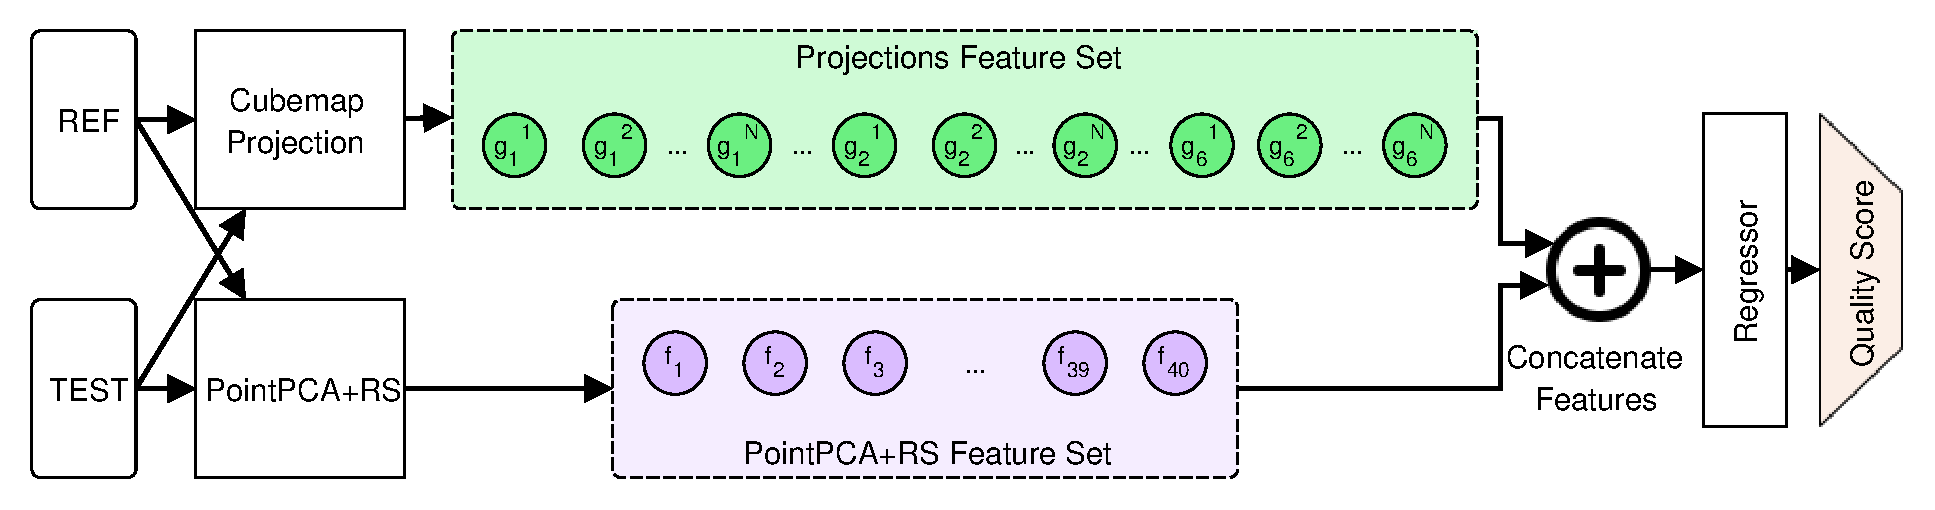
\includegraphics[width=\textwidth]{diagrams/pointpca3.pdf}
    \caption{Overall architecture of the proposed PointPCA++ metric. The reference and test PCs are used to obtain a Projections Feature Set via orthographic projections. Similarly, they are processed to generate the \gls{PointPCA+RS} feature set. Both feature sets are concatenated, and the result is used by a regression algorithm to predict a final quality score.}
    \label{fig_arquitecture_pointpca3}
\end{figure*}





\subsection{PointPCA+RS: PointPCA+ with Resource Streamlining} \label{sec_pointpca_rs}

Figure~\ref{fig_pointpca2_rs_diagram} gives an overview of \gls{PointPCA+RS}. A comparison of this figure with Figure~\ref{fig_pointpca2_diagram} reveals that both PointPCA+ and the proposed \gls{PointPCA+RS} share several common steps, including preprocessing, descriptor calculation, feature vector calculation, and a regression stage. The preprocessing stage involves two steps: duplicate merging and neighborhood identification. These steps, as explained in the previous section, serve to combine identical points by calculating the average color value for each point with multiple color values. However, while PointPCA+ utilizes a simple brute-force approach to find duplicates by comparing every point to all others, \gls{PointPCA+RS} employs a \texttt{BTreeMap}~\cite{muller2025b} to map each point to a vector containing all of its associated colors, including duplicates. The brute-force search used by PointPCA+, while it is a very simple and straightforward method, is also highly inefficient, especially for \glspl{PC} with large number of points. As the number of data points increases, the processing time and resource consumption rise significantly, making it slow and resource-intensive. In contrast, by using a \texttt{BTreeMap}, \gls{PointPCA+RS} organizes data in a hierarchical way, which makes it much faster to search for and retrieve information. In other words, instead of comparing every point, this data structure quickly maps each unique point to a list of its associated colors, including any duplicates. This significantly reduces the amount of work required and results in a much faster and more memory-efficient process.

To ensure highly efficient implementation of \texttt{BTreeMap}, we opted an opensource implementation of this data structure in Rust language. Consequently, due to this design choice, the whole backend of \gls{PointPCA+RS} was entirely developed in Rust~\cite{matsakis2014rust}. Leveraging the static typing and ownership-based memory management of Rust language, our implementation guarantees strong reliability and consistent performance by eliminating the need for garbage collection and minimizing memory usage through advanced memory modeling. By redefining sequential operations, \gls{PointPCA+RS} boosts computational efficiency by using parallelism and optimized data structures while maintaining the core principles of the original PointPCA+ algorithm. Specifically, \gls{PointPCA+RS} parallelizes the sequential steps of PointPCA+, focusing on the highly resource-demanding feature extraction steps.

The majority of the computational overhead is concentrated in the feature extraction phase (the steps inside the `Feature Extraction' group of Figure~\ref{fig_pointpca2_rs_diagram}). This is largely because of the extensive number of nearest neighbors searches that must be executed. For every point in the reference \gls{PC} $\mathcal{A}$, the algorithm identifies two sets of neighbors: the \glspl{KNN} within the reference itself and the \glspl{KNN} within the corresponding distorted \gls{PC} $\mathcal{B}$. This process is essential for creating a link between the local geometric areas in both \glspl{PC}.


PointPCA+ identifies local neighborhoods for each point in $\mathcal{A}$ by using the \texttt{knnsearch} function of Matlab~\cite{MATLAB}. While \gls{KNN} search is inherently resource-intensive, the PointPCA+ approach further amplifies these demands by pre-calculating all neighborhoods sequentially. This results in two $n \times k$ elements being stored in memory, where $n \in \{ \left| \mathcal{A} \right| \cup \left| \mathcal{B} \right| \}$ represents the number of points. For instance, with an reference \gls{PC} of 1 million points and a typical $k$ value of 81, the neighborhood arrays would each contain 81 million elements, resulting in a total of 162 million elements being allocated in memory before feature any feature calculations are performed.
 
\gls{PointPCA+RS} enhances computational efficiency by utilizing \texttt{kd\_tree} data structure available for Rust. This approach references the original point arrays without explicitly storing the neighborhoods, which effectively lowers the extra memory overhead from $O(nk)$ to $O(n)$. With the same aforementioned example, the 1 million points only require 2 million memory elements.
Moreover, in PointPCA+, during feature calculation, the algorithm iterate through each point, identify the local region using \gls{KNN}, performing \gls{PCA}, and then collect the features. This process involves significant redundancy, as  each point is examined individually. It is expected that even a single-point difference can lead to a substantial variation in the resulting features. On the other hand, in \gls{PointPCA+RS}, the \gls{KNN} of each point is collected and the inter-quartile range of the distances between point and its neighbors is computed. Points with distances below the inter-quartile range are marked as `visited' and processing continues. In subsequent iterations, if a `visited' point is found, that iteration is skipped and the the pre-computed distance is used. This statistical heuristic operates under the assumption that if point $a$ is within the neighborhood of point $b$, then point $b$ is also within the neighborhood of point $a$. While this is not universally true, it is sufficient to generate a feature set that is statistically similar to that produced by PointPCA+, as demonstrated in Section~\ref{sec_results}.

Furthermore, the construction process in \gls{PointPCA+RS} is parallelized, which drastically reduces the computation time needed for feature extraction stage. Subsequently, the local descriptors are computed in parallel for each neighborhood. This is done by spawning the processes through the points in $\mathcal{A}$ to compute the covariance matrix as outlined in Equation~\ref{eq_covariance_pointpca2}. Then, \gls{PCA} is performed on the covariance matrices of both $\mathcal{A}$ and $\mathcal{B}$  to find their eigenvectors and establish a local orthonormal basis. Using these bases, we can then compute features like the mean, variance, eigenvectors, and covariance for both geometric and texture data. 

\gls{PointPCA+RS} significantly improves efficiency by running iterations in parallel to calculate the $42 \times n$ descriptor matrix, similarly to described for Equations~\ref{eq_pooling_poinpca} and \ref{eq_pointpca2_feats}. Because each process is independent, it can extract neighborhoods from the pre-built \texttt{kd\_trees} as needed, compute descriptors, store the results in the descriptor matrix, and then free up memory. This approach is highly effective, especially since \glspl{PC} often contain millions or even billions of points. 

In the final feature vector computation stage, the descriptor matrix is processed to generate the predictors. In this stage, a pooling operation converts 42 descriptors into a set of 40 predictors. For a \gls{PC} with 1 million of points, PointPCA+ maintains in memory a descriptor matrix of dimensions 42$\times$1M and simultaneously a predictors matrix of dimensions 40$\times$1M, incurring huge memory usage. To address this problem, \gls{PointPCA+RS} computes the pooled predictors directly during the spatial metric calculation, avoiding the need to store the entire descriptors matrix. As each column of metrics is computed independently, they are immediately pooled into a $40 \times 1$ output vector, which significantly reduces the amount of memory used.


\subsection{Perception-Driven Quality Measurements of Cubemap Projections} \label{sec_cmp}

\begin{figure*}[t]
    \centering
    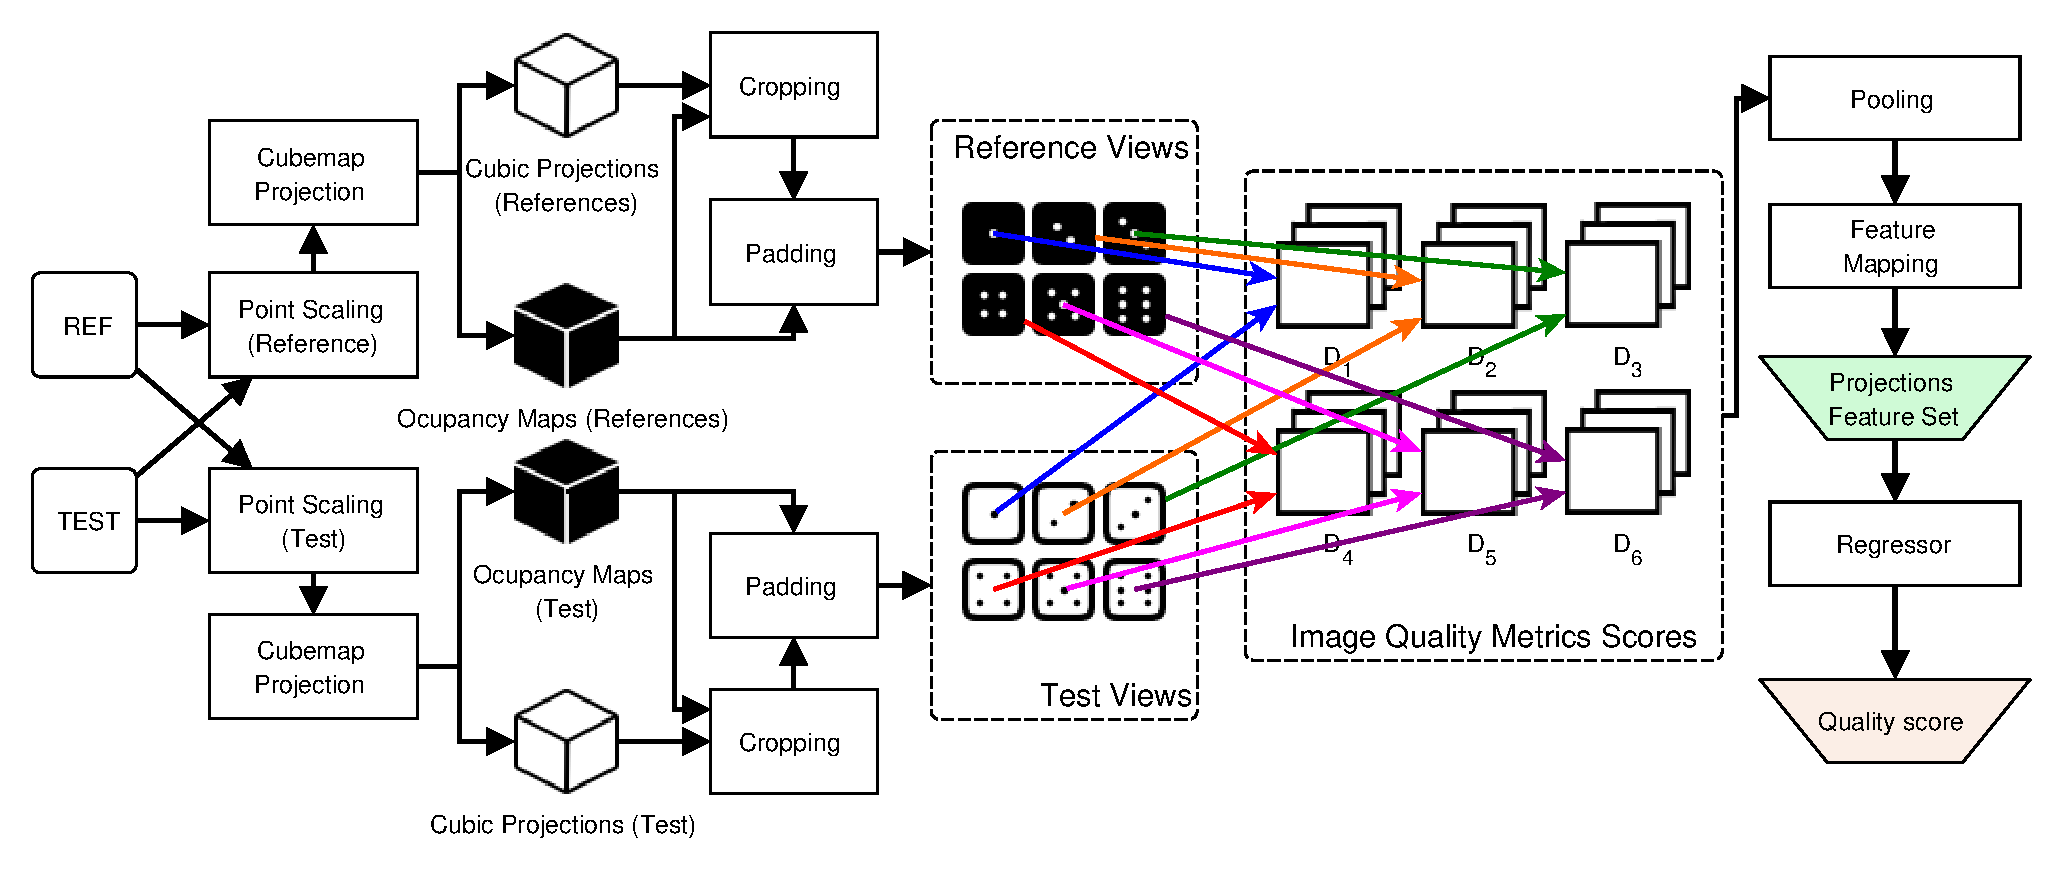
\includegraphics[width=\textwidth]{diagrams/orthographic_projections.pdf}
    \caption{Block diagram of the proposed projection-based PC metric. For PointPCA++, the projection feature set highlighted in green is used to model the metric.}
    \label{fig_arquitecture_orthographic_only}
\end{figure*}

Figure~\ref{fig_arquitecture_orthographic_only} depicts the block diagram of the proposed metric 3D-to-2D. It converts the original 3D \glspl{PC} onto six pairs of color texture and \gls{OcM}. Both reference and distorted \glspl{PC} are mapped to six perpendicular 2D image planes via \glspl{CMP}, as illustrated in Figure~\ref{fig_subemap}. The construction of \glspl{CMP} begins with point scaling processing to ensure consistency across samples. The point scaling ensures uniformity by shifting the \gls{PC} centroid to the origin and scaling the points such that their maximum distance
from the origin equals one. This step normalizes the points data, enabling uniform analysis across different samples. In other words, this process, performed in 3D space, ensures that the point data of the 3D representation will be aligned in the projected 2D space, thereby avoiding registration-related issues. 


\begin{figure}[t]
    \centering
    \begin{subfigure}[b]{.95\textwidth}
        \centering
        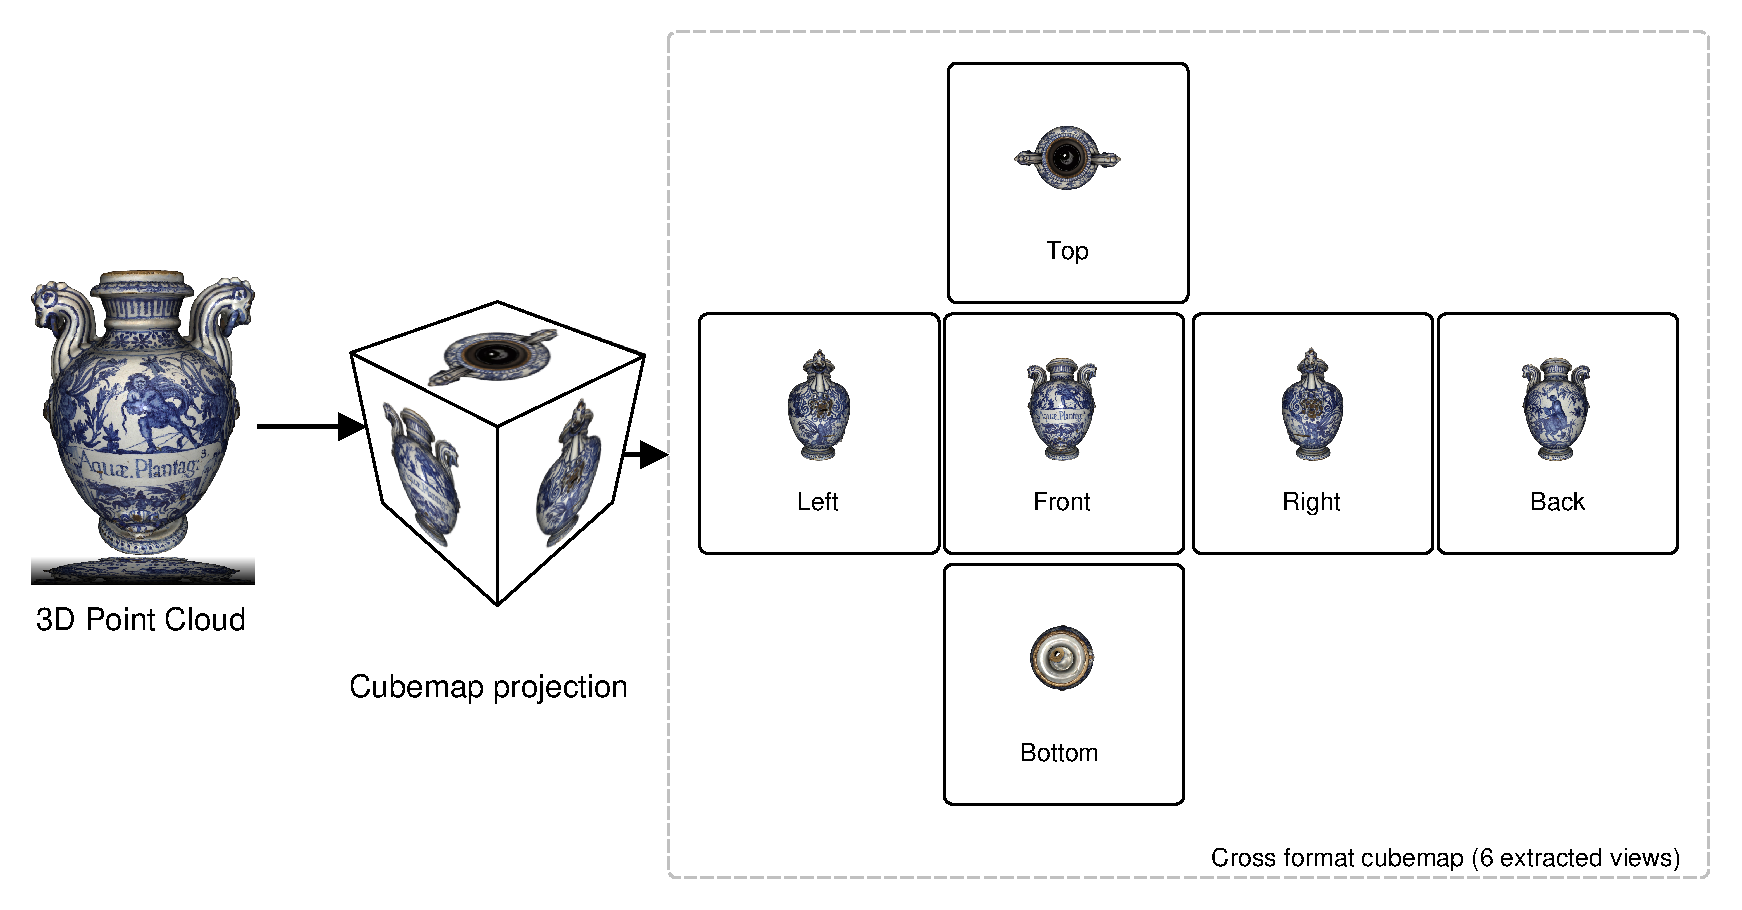
\includegraphics[width=\textwidth]{diagram_cubemaps/cubemap_views_generation.pdf}
        \caption{Six views generations}
        \label{fig_cubemap_generation}
    \end{subfigure}

    \begin{subfigure}[b]{.5\textwidth}
        \centering
        \includegraphics[width=\textwidth]{diagram_cubemaps/single_perspective_view.pdf}
        \caption{Single view representation}
        \label{fig_cubemap_single_view}
    \end{subfigure}
    \begin{subfigure}[b]{.3\textwidth}
        \centering
        \includegraphics[width=\textwidth]{diagram_cubemaps/perspective_mechanism.pdf}
        \caption{Perspective mechanism}
        \label{fig_cubemap_prspective_mechanism}
    \end{subfigure}

    \caption{Cubemap projection.}
    \label{fig_subemap}
\end{figure}


After point scaling, the 3D point cloud is first projected onto six perpendicular cubic faces, referred as the corresponding views, e.g., ``front view,'' ``back view,'' ``left view,'' ``right view,'' ``top view,'' and ``bottom view'', as shown in Figure~\ref{fig_cubemap_generation}. Each perspective
view has a 90 degree field of view both vertically and horizontally. The algorithm used to create a perspective projection begins by establishing a virtual camera at the origin. This camera's view is directed along the positive y-axis, with the z-axis serving as the ``up'' vector, as represented in Figure~\ref{fig_cubemap_single_view}. To generate a specific perspective view, one can rotate this initial camera's direction and orientation around any axis or a combination of axes. For a given coordinate system, a roll is a rotation around the y-axis, panning is a rotation around the z-axis, and tilting is a rotation around the x-axis. To generate the six faces of the cubemap, the initial camera's view direction is rotated accordingly, with both the horizontal and vertical fields of view set to 90 degrees. Considering the front as the initial viewpoint, the left view is obtained by panning 90 degrees, the right by panning -90 degrees, the back by panning 180 degrees, the top by tilting -90 degrees, and the bottom by tilting 90 degrees, as illustrated in Figure~\ref{fig_cubemap_prspective_mechanism}. 

When multiple points share the same x and y coordinates but have different z values, the point closest to the projection plane (i.e., the one with the smallest z value) is retained. It means that, depending from the viewpoint perspective, a point from \gls{PC} can be occupied in a given pixel of a view or not. By collecting all pixels corresponding to a projected point and assigning them a value of one, while leaving other pixels as zero, we create a binary image representing the \gls{OcM}. The resolution of the projected textures and \glspl{OcM} images are based on a `precision parameter' $\rho$, where the cube side is $2^\rho$.

The \glspl{OcM} are fundamental for subsequent steps, namely cropping and padding steps. These steps are illustrated in Figure~\ref{fig_cropping_and_padding_steps}. The cropping operation uses the \gls{OcM} to select the \gls{ROI} of the projected view. When a \gls{PC} is projected, a significant portion of the resulting image may consist of empty area, creating a background of non-occupied pixels that can interfere with the chosen \gls{IQA} technique. For instance, a pixel-level comparisons become unreliable because the non-degraded background contrasts with the occupied and degraded areas, leading to a poor correlation between objective metrics and subjective scores. To address this issue, \glspl{OcM} are employed to crop the projections, thereby reducing the background area and mitigating these effects.


\begin{figure*}[t]
  \centering
  \includegraphics[width=\textwidth]{diagrams/specific_projections_steps.pdf}
  \caption{Cropping and padding procedures applied to one out of the six projections.}
  \label{fig_cropping_and_padding_steps}
\end{figure*}




Even after cropping step, certain areas in the projected images still have empty information in relation to the original 3D data (unoccupied areas). These areas can still act as misleading element for \gls{IQA} algorithms and impairing their performance. To resolve this, we use an inpainting algorithm~\cite{telea2004image,bertalmio2001navier} to perform the padding operation. Inpainting involves filling in part of an image in a visually plausible way using information from the surrounding area. The idea comes from art restoration where damaged areas of paintings are ``inpainted'' to make them look complete again. Inpainting algorithms usually need the image to be inpainted and a mask. The mask tells the algorithm which parts of the image should be inpainted. Without a mask, the algorithm would not know the regions to replace. In this paper, we use the cropped \gls{OcM} as mask, as illustrated in Figure~\ref{fig_cropping_and_padding_steps}. In this figure, the white area of \gls{OcM} represents the portions of the image to be preserved, while the black area indicates the region to be inpainted.

\begin{figure*}[t!]
  \centering

  \includegraphics[width=\textwidth]{figures_inpaintings/fig_inpaints_algorithms.pdf}
  \caption{ Visual effects caused by inpainting algorithms on the different views.}
  \label{fig_inpainting_faces}
\end{figure*}



The padding operation is applied independently to both the pristine and distorted projections. This independent application ensures that the filled regions in the distorted view are not identical to those in the pristine one. Instead, they reflect the changes and shifts caused by the \gls{PC} degradation. Consequently, the final perceptual distance computed by the \gls{IQA} metric accurately captures the differences between the two images, including those within the filled areas, avoiding the potential for biased or misleading results. This approach allows our method to be robust against the sparsity of the \glspl{PC} while leveraging the strengths of existing 2D \gls{IQA}  techniques. 


\begin{figure*}[t!]
  \centering

  \includegraphics[width=\textwidth]{figures_inpaintings/fig_different_quality_levels.pdf}
  \caption{ Visual effects caused by inpainting algorithms on the same content impaired by different levels of the same distortion (DRACO lossy compression~\cite{de2022quality}).}
  \label{fig_inpainting_quality_levels}
\end{figure*}



\begin{figure*}[t!]
  \centering

  \includegraphics[width=\textwidth]{figures_inpaintings/fig_other_distortions.pdf}
  \caption{ Visual effects caused by inpainting algorithms on the same content impaired by  4 different compression algorithms (VPCC, GPCC-RAHT, GPCC-Predlift and GEOCNN) at varying compression levels as available in BASICS dataset~\cite{basics_dataset}.}
  \label{fig_inpainting_other_distortions}
\end{figure*}

Figures~\ref{fig_inpainting_faces}, \ref{fig_inpainting_quality_levels}, and \ref{fig_inpainting_other_distortions} illustrate the effects of the padding operation on projected point clouds. In this paper, we considered the Navier-Stokes-based~\cite{bertalmio2001navier}, Telea's~\cite{telea2004image}, \gls{FSR}~\cite{seiler2015resampling, genser2018signal}, and ShiftMap~\cite{shiftmap2012} inpainting algorithms. We chose these algorithms because they are relatively fast and publicly available through the OpenCV library. In Figures~\ref{fig_inpainting_faces}, shows the effects of these inpainting algorithms on the six projected views of a \gls{PC}. As can be noted, different algorithms produce different filling patterns. The images in the first column of Figures~\ref{fig_inpainting_faces} have different sizes due to the cropping operation. Figure~\ref{fig_inpainting_quality_levels} depicts the effect of padding on the same view perspective for point clouds impaired at different levels of degradation. Conversely, Figure~\ref{fig_inpainting_other_distortions} illustrates the effect of padding on pristine and distorted views with different types of distortions. It can be observed from these figures that padding produces distinct patterns for different distortion types and for different distortion levels of the same type.


After generating the cropped and padded projections, the next step involves computing a score per projection using one or more \gls{IQA} metrics, as illustrated in Figure~\ref{fig_arquitecture_orthographic_only}. For each \gls{IQA} metric used, a set of six scores is obtained, with each score corresponding to a pair of reference and assessed views. For example,  using a single  \gls{IQA} metric  yields the set of scores {$\{g_{0},g_{1},\cdots,g_5\}$} \gls{IQA}. When multiple metrics are employed, the scores are concatenated into a feature vector. Specifically, if $n$ etrics are used, the resulting feature vector is of size $6n$, represented as {$v = \{ g_{i} \}_{i=0}^{6 \times n}$}, where $g_j^k$ is score for view $j$ from the $k^{th}$ metric.

After generating the feature vector $v$, the rest of the pipeline is similar to that described for \gls{PointPCA+RS}. This is achieved using a regression algorithm, which takes $v$ as input and produces a quality score as output. To train this quality model, the feature vector is mapped to the subjective quality scores found in the quality databases, which can be expressed as $Q(I) = \mathfrak{R}(v, \mathcal{M})$, where $\mathfrak{R}(\cdot,\cdot)$ denotes the regression algorithm, $\mathcal{M}$ represents the trained regression model, and  $Q(\cdot)$ is the final predicted quality score of the assessed \gls{PC}.

\section{Experimental Setup} \label{sec_setup}

Benchmark datasets used to evaluate \gls{PCQA} metrics require perceptual quality values obtained from psychophysical experiments with human subjects.  In our tests, we use five datasets containing subjective scores collected from those experiments, as depicted in Table~\ref{tab_datasets}. These datasets are very diverse from each other and contain several \glspl{PPC}. Using these datasets to validate the effectiveness and reliability of the proposed \gls{PointPCA+RS}, we compare it with the original in terms of feature similarity, spent time, allocated memory, and correlations with \gls{MOS}.
All experiments were conducted on a system equipped with an AMD Ryzen Threadripper\texttrademark~2950X with 128GB RAM and  an NVIDIA GeForce GTX 1080TI\texttrademark~ graphics card.
{
 \def\arraystretch{1.3}
\begin{table}[t!]
  \centering
  \caption{Used Point clouds quality benchmark databases}

\adjustbox{max width=\columnwidth}
{
\begin{tabular}{c c c c >{\raggedright\arraybackslash}m{5cm} c c}
\toprule
DB & REF & Mnemonic & Attributes & Distortion & SRC & PPC \\
\midrule
D1       & \cite{apsipa_dataset} & \makecell{M-PCCD\\(APSIPA)} & Color & G-PCC, V-PCC & \centering 8 & 254 \\  \cdashline{1-7}[.4pt/1pt]

D2       & \cite{basics_dataset} & \makecell{BASICS\\(ICIP2023)} & \makecell{Color, Normals} & PCC, GPCC-RAHT, GPCC-Predlift and GEOCNN & \centering 75 & 1494 \\ \cdashline{1-7}[.4pt/1pt]

D3       & \cite{yang2020predicting} & SJTU-PCQA & Color & Octree, downsampling, color and geometry noise & \centering 9 & 378 \\ \cdashline{1-7}[.4pt/1pt]

D4       & \cite{Torlig2018anovel} & \centering UnB\_PC & \makecell{Color, Normals} & Octree, JPEG compression & \centering 6 & 60 \\ \cdashline{1-7}[.4pt/1pt]
D5   & \cite{wpc}     & WPC             & Color  & Gassian noise, dowsampling, G-PCC, V-PCC & \centering 20 & 740           \\
\bottomrule
\end{tabular}
}
\label{tab_datasets}
\end{table}
}


The method depicted in Figure~\ref{fig_arquitecture_pointpca3} was implemented in Python language, but some components of \gls{PointPCA+RS} and \gls{CMP} depicted in Figures~\ref{fig_pointpca2_rs_diagram} and \ref{fig_arquitecture_orthographic_only} where implemented in Rust language.
More specifically, as outlined in Sections~\ref{sec_pointpca_rs} and \ref{sec_cmp}, Rust was used to achieve performance and speed, particularly due to capacity for memory management and efficiency. Additionally, Rust uses a unique memory ownership model that enforces memory safety at compile time, guaranteeing no memory leaks or dangling pointers without the need for a runtime garbage collector. This leads to extremely low and predictable memory usage, which is critical for large \glspl{PC}. Rust was also chosen due to its capabilities for concurrency and parallelism. While Python's Global Interpreter Lock (GIL) limits true multi-threading in many cases, preventing multiple threads from executing simultaneously, the design of Rust language, particularly its ownership system, makes it safe and straightforward to write concurrent and parallel code without race conditions, allowing for highly efficient utilization of modern multi-core processors. Moreover, Rust's strict compiler and strong static typing catch a wide range of bugs at compile time that would normally only be found at runtime in Python (like type mismatches and memory-related errors). These properties help us to implement PointPCA++ in a more robust, reliable, and secure manner that is less prone to crashes.

Rust has a modern and robust tooling ecosystem centered around its package manager and build tool, Cargo. This makes it easy to manage dependencies and build projects. This means that the entire PointPCA++ project could be implemented in Rust. However, we opted for a polyglot approach, where the core implementation is done in Rust and the public interfaces are developed in Python, in order to leverage the advantages of both languages while avoiding their respective disadvantages. Specifically, Python as an huge community, with a vast collection of libraries for everything from data analysis and \gls{ML}. By providing a Python interface, our Rust-based core can seamlessly integrate into this rich ecosystem, making it far more accessible and useful to a broader researchers. 
The interoperability between Rust and Python components are integrated using PyO3/Maturin~\cite{johnson2024pyo3} that handles the complex data conversions between these two programming languages in a smooth interface.

We used the Lazypredict~\cite{lazypredict} as an initial test to determine the best suitable regression model. Lazypredict is a Python library designed to help with the evaluation and comparison of different Scikit-learn~\cite{scikit-learn} models. It automates the process of fitting multiple models to a dataset, making it easier to determine which models are likely to perform well without the need for extensive manual coding.
Additionally, \gls{SOTA} \gls{IQA} implementations were acquired from \gls{PIQ}~\cite{piq} and \gls{PyIQA}~\cite{pyiqa} libraries. 

The score prediction performance is measured using \gls{PLCC}, \gls{SROCC}, and \gls{RMSE}. These performance metrics are computed considering the predicted scores and the corresponding \gls{MOS} provided in the benchmark datasets. For learning-based methods, we used the Group K-fold with K=5, \gls{LOCO}, and grouped holdout validation techniques to split the data. In the case of grouped holdout validation, the  proportion of the splitting was defined to 80\% of groups for training and 20\% for testing. The groups are determined by the pristine (reference) content. In other word, for all these grouped validations, we exclude from training all observations that share the source reference (same content), i.e., \glspl{PPC} generated from a source reference in the test subset are not present in the training subset and vice-versa.




\section{Experimental Results} \label{sec_results}


This section examines the performance of the proposed PointPCA++ metric for subjective point cloud quality estimation. The components of PointPCA++ are first analyzed as independent metrics themselves, following the full pipelines depicted in Figures~\ref{fig_pointpca2_rs_diagram} and \ref{fig_arquitecture_orthographic_only}. Subsequently, the performance of these combined metrics, forming PointPCA++, is analyzed. The final step involves a comparison of PointPCA++ with \gls{SOTA} methods.



\red{Mencionar os datasets onde o MATLAB crashou}

\red{Mencionar os casos onde o MATLAB estourou a RAM}


\subsection{Performance comparison of PointPCA+ and PointPCA++}

\red{Aqui vão os gráficos, tabelas e análises comparando as performance (avaliação dos preditores, tempo e memória) do PointPCA2 original e da versão atualizada }

\red{OBS: NÃO USAR AS BASES DE DADOS QUE DÃO PROBLEMAS NESTA AVALIAÇÃO}




\subsection{Performance evaluation of predictors}

\red{Aqui vão uma analise de performance dos regressores e qual deles será escolhido para ser usado com a próxima sessão. Deve-se considerar também as features e parametros usados nas projeções (métricas do PIQ a serem usadas, etc). Cross-dataset, K-folds, etc, vão aqui.}

\red{COLOCAR FEATURE IMPORTANCES AQUI}



\subsection{Analysis of Projection Performance}



\subsection{Parallel Implementation Performance}


\red{Colocar umna análise aqui do ganho de performance ao se utilizar paralelização (aumentando o número de processo).}



\subsection{Comparison with the state-of-the-art}

\red{Aqui vão as tabelas e gráficos comparando o PointPCA++ proposto com outros métodos existentes.}


\section{Conclusion} \label{sec_conclusions}

\blue{Conclusão usada no WPOS2024 (expandir e melhorar)}

This paper proposes a novel type of \gls{PCQA} method that combines projection-based and \gls{PCA}-based techniques to predict the overall quality of \gls{PC} contents. Results show that the proposed approach outperform the independently-used techniques, showing robust and consistent prediction values that are well correlated with subjective quality scores, while requiring a fraction of the computation time and memory usage. Future works will investigate if the inclusion of saliency-aware descriptors can improve the the proposed metric performance.

\bibliographystyle{elsarticle-num} 
\bibliography{biblio}

\end{document}

\endinput
%%
%% End of file `elsarticle-template-num.tex'.
